\documentclass[conference]{IEEEtran}
\IEEEoverridecommandlockouts
% The preceding line is only needed to identify funding in the first footnote. If that is unneeded, please comment it out.
\usepackage{amsmath,amssymb,amsfonts}
\usepackage{algorithmic}
\usepackage{graphicx}
\usepackage{textcomp}
\usepackage{xcolor}
\usepackage{comment}
%\usepackage{todonotes}
\usepackage{wrapfig}
\usepackage{hyperref}
\usepackage{xurl}
\usepackage{booktabs}
\usepackage{float}
\usepackage[noadjust]{cite}

\def\BibTeX{{\rm B\kern-.05em{\sc i\kern-.025em b}\kern-.08em
    T\kern-.1667em\lower.7ex\hbox{E}\kern-.125emX}}
\begin{document}

\title{Automatic Metadata Generation for Fish Specimen Image Collections%*\\
    {\footnotesize \thanks{Research supported by NSF OAC \#1940233 and \#1940322.} }}

\author{
\IEEEauthorblockN{Joel Pepper}
\IEEEauthorblockA{\textit{Department of Computer Science} \\
\textit{Drexel University}\\
Philadelphia, PA\hspace{3mm}USA\\
\href{https://orcid.org/0000-0002-1601-8729}{0000-0002-1601-8729}}\\
\IEEEauthorblockN{Xiaojun Wang}
\IEEEauthorblockA{\textit{Biodiversity Research Institute} \\
\textit{Tulane University}\\
New Orleans, LA\hspace{3mm}USA\\
\href{https://orcid.org/0000-0002-2995-9050}{0000-0002-2995-9050}}
\and
\IEEEauthorblockN{Jane Greenberg}
\IEEEauthorblockA{\textit{Department of Information Science} \\
\textit{Drexel University}\\
Philadelphia, PA\hspace{3mm}USA\\
\href{https://orcid.org/0000-0001-7819-5360}{0000-0001-7819-5360}}\\
\IEEEauthorblockN{Henry Bart Jr.}
\IEEEauthorblockA{\textit{Biodiversity Research Institute} \\
\textit{Tulane University}\\
New Orleans, LA\hspace{3mm}USA\\
\href{https://orcid.org/0000-0002-5662-9444}{0000-0002-5662-9444}}
\and
\IEEEauthorblockN{Yasin Baki\c{s}}
\IEEEauthorblockA{\textit{Biodiversity Research Institute} \\
\textit{Tulane University}\\
New Orleans, LA\hspace{3mm}USA\\
\href{https://orcid.org/0000-0001-6144-9440}{0000-0001-6144-9440}}\\
\IEEEauthorblockN{David Breen}
\IEEEauthorblockA{\textit{Department of Computer Science} \\
\textit{Drexel University}\\
Philadelphia, PA\hspace{3mm}USA\\
\href{https://orcid.org/0000-0002-1376-5008}{0000-0002-1376-5008}}
}

\maketitle

%abstract can be shortened a good bit.
%can offer an alternative manana..
\begin{abstract}
Metadata is a key data source, particularly for researchers seeking to apply machine learning to the vast collections of digitized specimens. Unfortunately, the available metadata is often sparse and, at times, erroneous; and it is prohibitively expensive to address these limitations through traditional, manual means.
This paper reports on research that applies machine-driven approaches to
analyzing digitized fish images and extracting various of important
features from them. The digitized fish specimens are being analyzed as part of the Biology Guided Neural Networks (BGNN) initiative, which is developing a novel class of artificial neural networks using phylogenies and anatomy ontologies. Automatically generated metadata is crucial for identifying
the high-quality images needed for the neural network's predictive
analyses.
%predictive analytics?
Methods that  combine machine learning  and  image  informatics techniques allow us to rapidly enrich the existing metadata associated with each of the
7,244 images from the Illinois Natural History Survey (INHS). The sample
images each include 22 manually generated metadata properties, which
aid our study.  Results show we can  accurately generate metadata for
twenty key %6? 
metadata properties, for example: fish quantity, fish orientation,
image scaling based on
ruler identification and measurement, and general image quality metrics
(brightness and contrast). Results also show can also x, y, z.
%to confirm list of six properties.
%x, y, z = any other key results. jg will add from results section, unless someone else does first. 
The automatic process out-performs humans in terms of time and labor cost,
as well as accuracy, and provides a novel solution for leveraging digitized
specimens for machine learning. This research has implications for harnessing the tens of thousands of digitized specimens stored in open-access repositories found wold-wide.
%world wide [*across the globe] or we may not even need this part as open access is global access

% OLD text - Over the last several decades advances in computing, imaging, and cyberinfrastructure have had a major impact on scientific research and discovery. One area of considerable activity is the digitization of the biological specimens that have been acquired worldwide by museums and other research institutions, undertakings that have produced large image collections.The metadata that is vital for subsequent machine learning, analysis and scientific discovery based on these specimen image repositories is often unavailable, sparse or incorrect. As a step towards improving metadata in specimen research image collections, our team is developing methods for automatically analyzing fish images to extract a variety of important features. These fish specimens are being studied for a larger project entitled Biology Guided Neural Networks (BGNN), which is developing a novel class of artificial neural networks that can exploit the machine readable and predictive knowledge about biology that is available in specimen images, phylogenies and anatomy ontologies. Using a combination of machine learning and image informatics tools and techniques, we can accurately determine metadata such as fish quantity and location within images, fish orientation and other quantitative fish features, image scaling based on ruler identification and measurement, and general image quality metrics for a substantial number of the images being used in the BGNN project.Our goal is to develop image metadata generation methods that both support the research underway within the BGNN project, and provide a framework for future technology developments that can be deployed by repository curators to improve and bolster the metadata they provide with their specimen images. A longer term goal is to extend the image analysis methods for computing quantitative features in support of specific biological investigations.
\end{abstract}

\begin{IEEEkeywords}
bioinformatics, metadata, image analysis, applied machine learning
\end{IEEEkeywords}

\section{Introduction}
% Moving teaser since this template doesn't actually ask for one
Over the last several decades advances in computing, imaging, and cyberinfrastructure have supported the growth of digital natural history collections, many of which have specimen images~\cite{beaman2012mass}. Additionally, initiatives, such as the National Science Foundation’s Advancing Digitization of Biodiversity Collections (ADBC) program,
% (which ran for nearly a decade),
have supported the digitization and curation of tens of thousands of biological specimens~\cite{page2015digitization}. These digitized specimens are generally accessible through global, open-access repositories that support digital library services, such as browsing, search and retrieval, and preservation. The digitized renderings of these rich collections permit researchers, educators, students, and the general public to examine biological specimens
on a previously unattainable scale. Moreover, the digitized instantiations present a pathway for applying machine learning and making new scientific discoveries. 

Unfortunately, potential scientific advances are hindered by image quality
problems and the lack of accurate and pertinent metadata
associated with the image collections.
Poor quality images (e.g. low contrast, inadequate lighting,
out-of-focus or cluttered visual arrangements) provide inadequate input
for automated
image analysis and machine learning algorithms and lead to inferior
computational results.
In order to perform quantitative morphometric analysis of the specimens,
the physical scale of the images (pixels/inch) is needed; thus
requiring the ability to identify and measure rulers in the images.
Many specimen collections do include Darwin Core metadata~\cite{biodiv_info_standards}, detailing
specimen taxon, geographic location, and several other descriptive aspects.
Additionally, some digitization efforts record technical metadata, detailing imaging specifications. While these types of metadata are helpful for a
human examining several images at a time, they are insufficient for researchers seeking to apply computational methods %machine learning? or okay here
to examine thousands of images
to determine if, for example, a specific fish grows to different lengths
in different habitats, or the temporal evolution of an anatomical feature,
e.g.~the size of a dorsal fin.
\begin{figure*}
  \centering
  \includegraphics[width=.31\linewidth]{images/INHS_FISH_100314}
  \hspace{1mm}
  \includegraphics[width=.31\linewidth]{images/INHS_FISH_100682}
  \hspace{1mm}
  \includegraphics[width=.31\linewidth]{images/INHS_FISH_100020}
  \caption{Three example images from the Illinois Natural History Survey (INHS) collection.}
  \label{fig:INHS_examples}
\end{figure*}

Since digital collections may each contain tens of thousands of images, manually producing image-related metadata for each digitized specimen is both labor- and time-intensive and prohibitively expensive. Methods for automatically computing metadata are therefore needed to fully exploit biological image repositories for scientific discovery.
%we are both extracting and calculating. Just to double check then, our definition/understanding of computing here includes both of these, or should we focus on extraction, with the idea that calculating is the extra novel thing added, the application of math-the groovy stuff you guys added.  
As a step towards improving metadata in research specimen image collections, members of Drexel University's Metadata Research Center are developing methods to automatically analyze fish images and
extract a set of data features that provide important metadata about the
digitized specimens.
The research is being conducted as part of the Biology Guided Neural Networks (BGNN) project, which is developing a novel class of artificial neural networks that exploit machine readable and predictive knowledge associated with specimen images, phylogenies and anatomy ontologies.
Using a combination of machine learning and image informatics 
techniques,
%tools and [okay to just say image informatics techniques instead of "image informatics tools and techniques" - thinking techniques implies tools.]
we can accurately determine general image quality and metadata, such as fish quantity and location within images, fish orientation, and
image scaling based on ruler identification and measurement. Image scaling
allows us to compute quantitative features about the fish specimens, such
as their length and area.  In order to test and validate our methods, they
have been  applied to a set of \(7,244\)
images drawn from the Illinois Natural History Survey (INHS) Collection~\cite{INHS}.
Figure \ref{fig:INHS_examples} presents three typical images used in our
study.
%Dave/Joel, the section above, from "we can accurately ..." to the figures" to me is more results. I guess it's okay to give this in introduction. Just wanted to raise this point. I sometimes give a paraphrase too, but just good to see if it is a little too much or okay with you both. I think it's okay as I re-read it, but good to have someone check.
The following section of the paper provides contextual background for this work, followed by the research goals and objectives, and a review of our research methods. Next, the results, along with discussion, are presented. The conclusion highlights key findings and identifies next steps.

\section{Related Work}
\subsection{Metadata for Natural History Image Collection}
%question/comment - we need to keep in mind we are deal with digitized specimens, not simply digital, in other words, the artifacts themselves are digital version of physical, not like an x-ray, where the image is digital from the start.  
A number of different metadata standards have been applied to support the description and access of digitized scientific images. The Darwin Core (DwC)~\cite{biodiv_info_standards}, developed specifically to describe biological diversity data, is one of the most popular standards for such efforts. It is an extension of the Dublin Core's DCMI Metadata Terms~\cite{dc_terms}.
The Audubon Core~\cite{audub_core}, which supports the discoverability, dissemination, and use of data related to biological organisms (including 3--D digitized specimens), is a DwC extension that has become more popular. All of these descriptive standards and extensions include metadata properties for taxon, geographic location, and other important specimen content, and have been developed primarily from the perspective of a human curator. In other words, their application anticipates that a curator or data entry staff will manually generate metadata, drawn from acquisition logs or original specimen labels. This task is labor intensive, and the metadata associated with each digital rendering is generally sparse and more prone to human error, placing limitations on a researcher seeking to apply machine learning to the image and the metadata for scientific research.

This limitation is magnified when trying to assess the actual quality of the digitized specimen. Descriptive-oriented standards support search and retrieval, and the biodiversity community has advocated for data fitness standards \cite{chapman2020developing}. This point is also emphasized by
Wieczorek et al.~\cite{wieczorek2012darwin} in their report on the variety of DwC metadata extensions needed to meet growing community concerns and
requirements, including data quality and fitness. Even so, metadata describing image quality is severely limited and generally missing. This point is addressed in detail by Leipzig et al.~\cite{leipzig2021biodiversity} and serves as the rationale for Tulane University's effort to manually capture
content for 22 metadata properties that characterize digitized specimen image quality. Their work is being conducted in connection with the larger BGNN initiative, and the current process is costly in terms of labor and time, prone to human error and inconsistencies, and underscores the need to
explore automatic metadata generation methods.
%Fish species dataset in Pakistan Shah 2019 \cite{Shah2019FishPakFS}
\subsection{Automatic Metadata Generation}
Automatic metadata generation advances covering both descriptive and technical metadata are relevant to the research presented in this paper. Automatic metadata generation of descriptive bibliographic data has been a research focus for close to 20 years \cite{liddy2002automatic,greenberg2004metadata,cardinaels2005automating,paynter2005developing}. Researchers have applied support vector machine (SVM) approaches~\cite{han2003automatic}, and associated networks to address sparse and incomplete metadata~\cite{rodriguez2009automatic}, and various successes are integrated into day-to-day workflows. Heidorn, et al.~\cite{heidorn2008automatic} demonstrated the use of optical character recognition (OCR) to extract specimen information from the original typed and often hand-annotated labels that are digitized along with herbarium collection holdings. The extracted information was encoded in the DwC metadata associated with the specimen's digitized rendering. There has also been some success with extracting descriptive cartographic information from maps~\cite{manso2004automatic}. While descriptive metadata covers taxon, geographic location, and other important aspects, and may even record the image format; extensive use of automatic processes are still limited. More significantly, descriptive metadata does not sufficiently addressed data quality.

Technical metadata, such as camera settings and temporal information (date and time) are automatically generated during a digitization sequence, following standards such as Exchangeable image file format (Exif)~\cite{Exif}. The camera's technical metadata is automatically captured and inserted into digital image files at the time of acquisition. Some of this metadata may be useful when selecting a machine learning sample. A researcher may desire images with specific properties, such as being captured chiefly with a certain aperture setting. Even so, the majority of automatically registered technical metadata associated with digitized specimens is also insufficient for computational research, leaving researchers to rely on manually generated descriptive metadata, which itself is sparse and prone to human error.
Fish image analysis research, as reviewed below, demonstrates the
potential of automated computational methods to address current metadata shortcomings and needs specific to the selection of high-quality digitized specimen images for the application of machine learning.

\subsection{Fish Image Analysis}

Image analysis has been utilized to examine and process images of fish
for well over two decades~\cite{Zion2000InvivoFS,Saberioon2017ApplicationOM}. It is an important
application of technology both for marine science, in the study of aquatic
species, habitats and ecosystems, and for the seafood industry, in the
development of automated fish sorting and grading systems, as well as
fisheries management. Many of these computational analyses focus on
the recognition and classification
of the fish present in an image.  The computational methods employed for
fish image analysis have followed the general trends in the AI field.
Hu et al.~\cite{HuJing2012Fscb} presented a method of classifying species
of fish based on color and texture features and a multi-class support
vector machine (MSVM)~\cite{Vapnik1999AOS}.
Li and Hong~\cite{Li2014IdentificationOF} computed eleven shape and color
features from fish images and derived a linear model
that could discriminate between four different fishes.
%  Kinda unimpressive. Let's leave out.
% Saitoh \cite{Saitoh2015ImagebasedFR}
% utilized a Random Forest method \cite{Breiman2001RF} on manually-derived
% geometric, Bag of visual words (BoVW) and color features 
Rodrigues et al.~\cite{RodriguesMarcoT.A2015Ecda} explored several
combinations of features extraction, input classifiers and clustering
algorithms to produce a method that could distinguish between 10 different
types of fish with a 92\% accuracy.
%  Again, not too impressive. Let's leave out.
% Ogunlana 2015 \cite{Ogunlana2015FCU},
% In this paper, a Support Vector Machine (SVM)-based technique for the elimination of the limitations of some existing techniques and improved classification of fish species is proposed. The technique is based on the shape features of fish that was divided into two subsets with the first comprising 76 fish as training set while the second comprises of 74 fish as testing set. The body and the five fin lengths; namely anal, caudal, dorsal, pelvic and pectoral were extracted in centimeter (cm). Results based on the new technique show a classification accuracy of 78.59%, which is significantly higher than what obtained for ANN, KNN and K-mean clustering-based algorithms.
Salman et al.~\cite{Salman2016FishSC} employed a deep Convolution Neural
Networks (CNN) \cite{LeCun2004LMG} together with classification based on
K-Nearest Neighbor and Support Vector Machines trained on the features
extracted by the CNN. They achieved 90\%
accuracy when identifying 15 different fish in challenging underwater
digital images.
% Unimpressive. Do not include.
% Sung 2017 \cite{Sung2017VisionBR},
% Underwater vision has specific characteristics such as high attenuation of lights, severe noise and haze in the images. For real-time fish detection using underwater vision, this paper proposes convolutional neural network based techniques based on You Only Look Once algorithm. Actual fish video images were used to evaluate the reliability and accuracy of the proposed method. As a result, the network recorded 93% classification accuracy, 0.634 intersection over union between predicted bounding box and ground truth, and 16.7 frames per second of fish detection. It also outperforms another fish detector using sliding window algorithm and classifier trained with histogram of oriented gradient features and support vector machine.
% Not digging it.
% Hasija 2017 \cite{Hasija2017FishSC},
% This paper proposes a novel method based on an improved image-set matching approach, which makes use of Graph-Embedding Discriminant Analysis. In contrast to the state-of-the-art methods, which operate on single input images, our method makes, use of explicit image set matching which renders it robust computationally.
% Not this one either
% Sayed 2018 \cite{SayedGehadIsmail2018AAFS},
% This paper proposed an automated fish species identification system based on a modified crow search optimization algorithm. Median filtering is applied for image smoothing and removing noise through reducing the variation of intensities between the neighbors. Then, a k-mean clustering algorithm is used to segment the fish image into multiple segments. Shape-based and texture-based feature extraction process for classification is presented. A new modified binary version of crow search algorithm is proposed to reduce the data dimensionality of the extracted features. Finally, support vector machine and decision trees are implemented for classification and the fish species are classified based on either their class including Actinopterygii and Chondrichthyes or based on their order. Total of 270 images with different species, classes and orders are used for evaluation of the proposed system. The experimental results show that the proposed system achieves the highest classification accuracy compared to state-of-the-art algorithms. Also, the results show that the overall fish species identification system obtains on average of 10 folds, 96% classification accuracy for classification based on class and 74% for classification based on fish order.
Utilizing texture, anchor points, and statistical measurements,
Alsmadi et al.~\cite{Alsmadi2019RFE} implemented fish classification
through a meta-heuristic algorithm known as the Memetic Algorithm.
% (Genetic Algorithm with Simulated Annealing) with back-propagation algorithm (MA-B Classifier).
They were able to classify 24 fish families with 90\% accuracy.
% Nope
% Sharmin 2019 \cite{Sharmin2019MVB},
% the new generation people of Bangladesh lacks the knowledge of local freshwater fish. For this problem, a solution has been found with the collaboration of vision-based technology. As a solution, a machine-vision based local freshwater fish recognition system is presented that can be proceed with an image of fish captured with a mobile or handheld device and recognize the fish in order to introduce the fish. To demonstrate the utility of the proposed expert system, several experiments are performed. At first, a set of fourteen features, which consists of four types of features, are presented. Then the color image has been converted into gray-scale image and the gray-scale histogram is formed. Image segmentation takes place using histogram-based method and then the features are extracted. PCA is used for decreasing the feature numbers. Three classifiers are used for recognizing fish, where SVM gives the highest accuracy showing a value of 94.2%.
%  I want to see the paper before I cite it.
% Banan 2020 \cite{Banan2020DeepLA}
% Hence, in this study, a deep learning neural network as a smart, real-time and non-destructive method was developed and applied to automate the identification of four economically important carp species namely common carp (Cyprinus carpio), grass carp (Ctenopharingodon idella), bighead carp (Hypophtalmichthys nobilis) and silver carp (Hypophthalmichthys molitrix). The obtained results proved that our approach, evaluated through 5-fold cross-validation, achieved the highest possible accuracy of 100 %. The achieved high level of classification accuracy was due to the ability of the suggested deep model to build a hierarchy of self-learned features, which was in accordance with the hierarchy of these fish’s identification keys. In conclusion, the proposed convolutional neural network (CNN)-based method has a single and generic trained architecture with promising performance for fish species identification.
Iqbal et al.~\cite{Iqbal2021AutomaticFS} used a modified
AlexNet \cite{AlexNet2012} model to classify six different fish species
with 90\% accuracy.
% In this paper, we presented an automated system for identification and classification of fish species. It helps the marine biologists to have greater understanding of the fish species and their habitats. The proposed model is based on deep convolutional neural networks. It uses a reduced version of AlexNet model comprises of four convolutional layers and two fully connected layers. A comparison is presented against the other deep learning models such as AlexNet and VGGNet. The four parameters are considered that is number of convolu- tional layers and number of fully-connected layers, number of iterations to achieve 100% accuracy on training data, batch size and dropout layer. The results show that the proposed and modified AlexNet model with less number of layers has achieved the testing accuracy of 90.48% while the original AlexNet model achieved 86.65% over the untrained bench- mark fish dataset. The inclusion of dropout layer has enhanced the overall performance of our proposed model. It contain less training images, less memory and it is also less compu- tational complex.
%  No paper. No reference
% Xu 2021 \cite{Xu2021TransferLA},
% Scientific studies on species identification in fish have considerable significance in aquatic ecosystems and quality evaluation. The morphological differences between different fish species are obvious. Machine learning methods use artificial prior knowledge to extract fish features, which is time-consuming, laborious, and subjective. Recently, deep learning-based identification of fish species has been widely used. However, fish species identification still faces many challenges due to the small scale of fish samples and the imbalance of the number of categories. For example, the model is prone to being overfitted, and the performance of the classifier is biased to the fish species of most samples. To solve the above problems, this paper proposes a fish species identification approach based on SE-ResNet152 and class-balanced focal loss. First, visualization analysis and image preprocessing of fish datasets are carried out. Second, the SE-ResNet152 model is constructed as a generalized feature extractor and is migrated to the target dataset. Finally, we apply the class-balanced focal loss function to train the SE-ResNet152 model, and realize fish species identification on three fish image views (body, head, and scale). The proposed method was tested on the Fish-Pak public dataset and achieved 98.80%, 96.67%, and 91.25% accuracy on the three fish image views, respectively. To ensure the superior performance of the proposed method, we performed an experimental comparison with other methods involving SENet154, DenseNet121, ResNet18, ResNet152, VGG16, cross-entropy, and focal loss. Comprehensive empirical analyses reveal that the proposed method achieves good performance on the three fish image views and outperforms common methods.


% \textbf{Orientation, Length, Size, Weight and Shape}\newline
Especially in industrial settings, it is necessary to automatically
detect the orientation, length and weight of fish during handling
and processing.
In some instances fish in the images need to be computationally straightened
before further processing can be attempted \cite{MuozBenavent2018EnhancedFB}.
Balaban et al.~\cite{Balaban2010UsingIA} demonstrated that image analysis
and data fitting may be used to predict the weight of salmons with high
accuracy.
% After harvesting , salmon is sorted by species, size, and quality. This is generally manually done by op-erators. Automation would bring repeatability, objectivity, and record-keeping capabilities to these tasks. Machinevision (MV) and image analysis have been used in sorting many agricultural products. Four salmon species weretested: pink (Oncorhynchus gorbuscha), red (Oncorhynchus nerka), silver (Oncorhynchus kisutch), and chum (On-corhynchus keta). A total of 60 whole fish from each species were first weighed, then placed in a light box to taketheir picture. Weight compared with view area as well as length and width correlations were developed. In additionthe effect of “hump” development (see text) of pink salmon on this correlation was investigated. It was possible topredict the weight of a salmon by view area, regardless of species, and regardless of the development of a humpfor pinks. Within pink salmon there was a small but insignificant difference between predictive equations for theweight of “regular” fish and “humpy” fish. Machine vision can accurately predict the weight of whole salmon forsorting.
% Konovalov 2017 \cite{KonovalovD2017RDfA},
% Fast and low cost image collection and processing is often required in aquaculture farms for quality/size attributes and breeding programs. For example, the absolute physical dimensions of fish (in millimeters or inches) could be estimated from electronic images. The absolute scale of the photographed fish is often unknown or requires additional hardware, data- collection and/or management overheads. One cost and time effective solution is to capture the absolute scale (in pixels-per- millimeter or dots-per-inch) by including a measuring ruler in the photographed scene. To assist that type of workflow, we designed a relatively simple image-processing algorithm that automatically located a sufficiently large section of the ruler in a given image. The algorithm utilized the Fast Fourier Transform and was designed to be free from adjustable parameters and therefore did not require training or calibration. The algorithm was tested on 445 images of Barramundi (Asian sea bass, Lates calcarifer), where a millimeter-graded ruler was included in each image. The algorithm achieved precision of 98% (on the original, 10, 20, 70, 80 90 degree rotated images) and 95-96% on 40, 50, 60 degree rotated images. \newline
% Konovalov 2018 \cite{Konovalov2018AutomaticSO},
% Approximately 2,500 weights and corresponding images of harvested Lates calcarifer (Asian seabass or barra- mundi) were collected at three different locations in Queensland, Australia. Two instances of the LinkNet-34 segmentation Convo- lutional Neural Network (CNN) were trained. The first one was trained on 200 manually segmented fish masks with excluded fins and tails. The second was trained on 100 whole-fish masks. The two CNNs were applied to the rest of the images and yielded automatically segmented masks. The one-factor and two-factor simple mathematical weight-from-area models were fitted on 1072 area-weight pairs from the first two locations, where area values were extracted from the automatically segmented masks. When applied to 1,400 test images (from the third location), the one- factor whole-fish mask model achieved the best mean absolute percentage error (MAPE), MAPE = 4.36%. Direct weight-from- image regression CNNs were also trained, where the no-fins based CNN performed best on the test images with MAPE = 4.28%.
Hao et al.~\cite{Hao2015TheMO} provide an excellent review of fish
measurement efforts that utilize machine vision.
% This study reviewed the methods of fish size measurement through machine vision. Length and area are important information that can help fishers manage fish scientifically and conveniently. This information could be used to calculate the volume and weight according to their relation; other information could also be calculated. Machine vision is more effective, economical and faster than traditional methods.
Azarmdel et al.~\cite{Azarmdel2019DevelopingAO} developed a system
capable of determining the orientation of a trout and segmenting its fins,
which are used as cutting points, with an accuracy over 99\%.
% Fish processing in small and medium fish supplying centers requires an intelligent system to operate on different sizes. Therefore, an image processing algorithm was developed to extract the proper head and belly cutting points according to the trout dimensions. The algorithm detects the fish orientation and location of pectoral, anal, pelvic, and caudal fins. In this study, each of the trout images was divided into slices along its length in order to segment the fins and extract cutting points. The channel ‘B’ of RGB color space was considered in both initial segmentation and fin detection stages among the examined channels of RGB, HSV, and L*a*b* color spaces. The back-belly and head-tail sides were detected with an accuracy of 100% based on gray intensity values and head to tail ratio, respectively. Furthermore, performing an analysis of variance (ANOVA) resulted in an F-value of 64.82 among the fins. Conducting a t-test among the mean intensity values of the fins and non-fin regions of channel ‘B’ resulted in the highest distinction with t-values of 90.30, 78.07, 74.28, and 86.01 with p < 0.01 for the pectoral, pelvic, anal, and caudal fins paired with the corresponding non-fin region, respectively. The results showed that the selected ‘B’ channel is the adequate one for fin segmentation. The fin detection process showed an overall sensitivity, specificity, and accuracy of 86.05%, 99.97%, and 99.87%, respectively. By solving the line determination error in 8.24% and the extra object error in 4.12% of the samples, the overall fin identification accuracy was 100%. Finally, after extracting the fin regions, the start point of the pectoral fin and the end point of the anal fin will be applied in the trout processing system as the head and belly cutting points, respectively.
Another application of image analysis to fish images is the evaluation of
fish freshness, a computation usually performed on the color features of
the images.
Tappi et al.~\cite{Tappi2017ComputerVS} assess the freshness of frozen
fish by computing a change of color and an eye concavity index.
% The evaluation of fish freshness can be per- formed using chemical, sensory and physical methods. Besides sensory methods, several instrumental techniques have been applied with the objective of replacing sensory assessment. The aim of this study was to set up and test objective physical methods mainly based on computer vision system (CVS) to assess red mullet (Mullus barba- tus) freshness evolution during 10 days of storage, at two different storage temperatures (0 and 4 °C). To check the effectiveness of the purposed physical methods, CVS fea- tures (loss in the epidermis pigmentation, development of gill mucus and eye concavity index) and firmness have been compared with chemical trimethylamine content and sensory (QIM) attribute scores. As expected, fish degrada- tion was faster at the higher temperature. Instrumental tex- ture evaluation of fish by penetration test enabled to detect distinctive firmness changes due to onset and resolution of rigor mortis, and the successive tenderization phenomenon. Among CVS parameters, the epidermis pigmentation loss, and particularly the eye shape modification (eye concavity index) evidenced a high sensibility for the estimation of fresh red mullet quality loss, as a function of the two differ- ent storage conditions, and a good agreement with trimeth- ylamine content and QIM response evolution.
Taheri-Garavand et al.~\cite{TaheriGaravand2019RealtimeNM} diagnosed the
freshness of common carp during ice storage. They utilize color feature
extraction and Artificial Neural Networks (ANN) to place fish in four
freshness categories with 93\% accuracy.
% In the current research, the potential of a novel method based on the artificial neural network was investigated to diagnose the freshness of common carp (Cyprinus carpio) during ice storage. Fish as an aquaculture product has high nutrients and low-fat content. So, people have consumed it as a safe and high-value foodstuff in their daily diet. Investigation of fish freshness is proposed as a significant issue in the aquaculture industry since fish spoils rapidly. The applied system of this study is comprised of the following steps: First, images of samples were captured and the pre-processing operation was done on the images. Then, particular channels including R, G, B, H, S, I, L*, a*, and b* were computed. Next, feature extraction was performed to obtain 6 types of texture features from each channel. Afterward, the hybrid Artificial Bee Colony-Artificial Neural Network (ABC-ANN) algorithm was applied to select the best features. Finally, the Support Vector Machine (SVM), K-Nearest Neighbor (K-NN) and Artificial Neural Network (ANN) algorithms as the most common methods were used to classify fish images. The best performance of the K-NN classifier was calculated in the k = 8 neighborhood size with the accuracy of 90.48. The best kernel function for the SVM algorithm was polynomial with C, sigma, and accuracy of 1, 2 and 91.52 percent, respectively. In this system, the input layer has consisted of 22 neurons based on the feature selection operation and 4 classes including most fresh, fresh, fairly fresh and spoiled have been used as the number of output layer. At the end, the best results of the MLP networks were achieved by LM learning algorithm and 6 neurons in the hidden layer with the 22–10–4 topology and accuracy of 93.01 percent.
% The achieved results demonstrate the high performance of the ANN classifier for evaluation of common carp freshness during ice storage as a rapid, accurate, non-destructive, real-time and automated method. It shows the potential of computer vision method in combination with artificial neural networks as an intelligent technique for evaluation of fish freshness.
A similar approach was developed by Lalabadi et al.~\cite{Lalabadi2020FishFC}.


The research reviewed above involves image features extraction and
artificial intelligence; although the researchers have not applied these
approaches to the burgeoning collections of digitized specimens
accessible in open repositories. Our research addresses this need by
applying machine learning and image informatics techniques to extract key
metadata properties from fish specimen images and computing
higher-level metadata based on these initial results.
Our goals and objectives our presented below.

\begin{comment}
Our work stands apart from previous work in that we are
addressing a different need: lack of metadata is impeding scientific studies.
Our focus and motivation are different.
Effectively doing the computational pre-processing
that will enable further downstream analyses.

<--NOTE-NOTE-NOTE DAVE/JOEL/ALL - RE: above paragraph, I'm thinking we should we shift message a little bit to something like, e.g., "The research reviewed above demonstrates image features extraction; although researchers have not applied these approaches the rich and extensive collections of digitized specimens accessible in open repositories. Our research addresses this need by applying machine learning and informatics techniques to extract key metadata properties from the images, and, further computing higher-level metadata based on these initial results. Our goals and objectives are presented in the following section.
\end{comment}

%I think this paragraph could be deleted then, or moves elsewhere, we say this a lot already: We are applying a variety of machine learning, image processing and image informatics techniques to extract key metadata properties from the images. These properties a critical for selecting high-quality, usable digitized specimens for further computational analysis, and and ensuring that the specimen images meet both scientific and technical requirements.


% Developing new techniques to determine fish freshness and quality can enhance nutritional value of the overall household food basket. In this research, digital image analysis was utilized to assess the freshness of rainbow trout fish by tracing the color attributes of its eyes and gills. The image data were collected from left and right eyes and gills in a 10-day ice-storage duration, and color components were extracted in RGB, HSV, and L*a*b* color spaces. Analysis of variance revealed that the RGB components of both eyes and gills had a significant change towards getting brighter during the ice-storage. Feature extraction was fulfilled from the color spaces, and then artificial neural networks (ANNs) and support vector machines (SVMs) were applied for classification of the ice-storage durations. The overall accuracies of the developed models demonstrated that the ANN somewhat outperformed the SVM for both the extracted features from the eyes and gills. Moreover, the gills’ features could describe the variance in the storage durations more efficiently than those extracted from the eyes. Finally, it was concluded that the applied colorimetric system along with the developing models could be employed as a successful non-destructive approach for evaluation of fish freshness.

\begin{comment}
\textbf{Not Used}\newline
(Kinda vague. More about food, then fish, G{\"u}m{\"u} 2011 \cite{Gm2011MachineVA}),
(In Turkish, Iscimen 2014 \cite{Iscimen2014ImageAM},
Iscimen 2015 \cite{Iscimen2015ClassificationOF}),
(Not based on images (sonar?) Kinjo 2014 \cite{KinjoAtsushi2014Scoi}),
(Too basic, Wang 2015 \cite{Huihui2015StudyOT}),
(Not so interesting, a very engineered, constrained imaging set up, Miranda 2017 \cite{MIRANDA201741}),

(A review of all types of sensing systems for quality checkin, Bernardo 2020 \cite{Bernardo2020FishQI}),
(Another review, but in Trends in Analytical Chemistry. I think we can
skip it. Not so technical, Dowlati 2012 \cite{Dowlati2012ApplicationOM}),

(Simple industrial system. Computing length, Sung 2020 \cite{Sung2020AutomaticGF}),

(These are 3D. Don't want to go there, Bock 2018 \cite{BockAlexander2018TITE},
Williams 2020 \cite{Williams:2020:UIF})

(A review that is not quite focused enough, Petrov 2020 \cite{Petrov2020Overview}),
(Don't have access to it, and I have a newer review, Zion 2012 \cite{Zion2012ReviewTU}),
\end{comment}



\section{Goals and Objectives}

Digitized specimens accessible in open-access repositories provide a rich,
extensive data source for machine learning and scientific discovery.
These resources, however, remain largely untapped due to image quality
issues and metadata limitations.
The overall goal of our work addresses this need by
% combining machine learning and image informatics techniques to produce
developing a computational
% . The overall goal of our research is to offer a machine-driven [*novel/innovative?? blah...]
alternative to the current manual metadata generation process, one that is
prohibitively costly in both terms of labor and time. Additionally, our
methods collectively provide a novel and general approach to computing
higher-level metadata that will support scientific inquiry based
on the analysis of specimen image collections.


% [WHAT'S THE DIFFERENCE BETWEEN A GOAL AND AN OBJECTIVE?]

Our four key objectives are to:

1) Explore use of Facebook AI Research's \verb|detectron| tool.  Specific
aims are to use \verb|detectron| to identify study-specific objects.
% classes: fish, fish eyes, rulers, and the numbers 2 and 3 on rulers, as shown in
% Figure \ref{fig:teaser}.

2) Investigate image processing at the pixel level.
Pilot testing found that \verb|detectron| under-segmented the detected objects
with tightly enclosing bounding boxes. We will determine if
pixel analysis methods commonly found in image informatics may produce
more accurate bounding boxes and object masks.
% background as part of the fish, or the
% bounding box may clip away part(s) of the fish with
The specific aims of this objective are to:
%not sure we have to list all the details, but something like the below, with the 4 aspects of pixel analysis we tested/investigate/experimented with

\renewcommand{\labelenumi}{\alph{enumi}.}
\begin{enumerate}
\item
Identify the appropriate threshold value for a more accurate mask.
% We will compute optimal scaling between [*or is it Otsu thresholding] to identify an improved threshold value. [Or we will determine is we can computed as the halfway point between the Otsu threshold value and the mean of the background intensities.]

\item
Remove noise to produce a single, solid mask.

\item
Compute a more accurate bounding box from the updated mask.
% Adjusting the bounding box. [We will use computational methods for masking [calcuate a mask?] to determine if bounding box needs to be shrunk or expanded]
% Jane confused here, if this belongs here, or below

\item
Automatically determine when modified methods fail and detectron values
should be used as is.
% Developing a fallback approach for when flood fill operations behave unexpectedly the image is too washed out.
\end{enumerate}

\begin{figure*}[t]
  \centering
 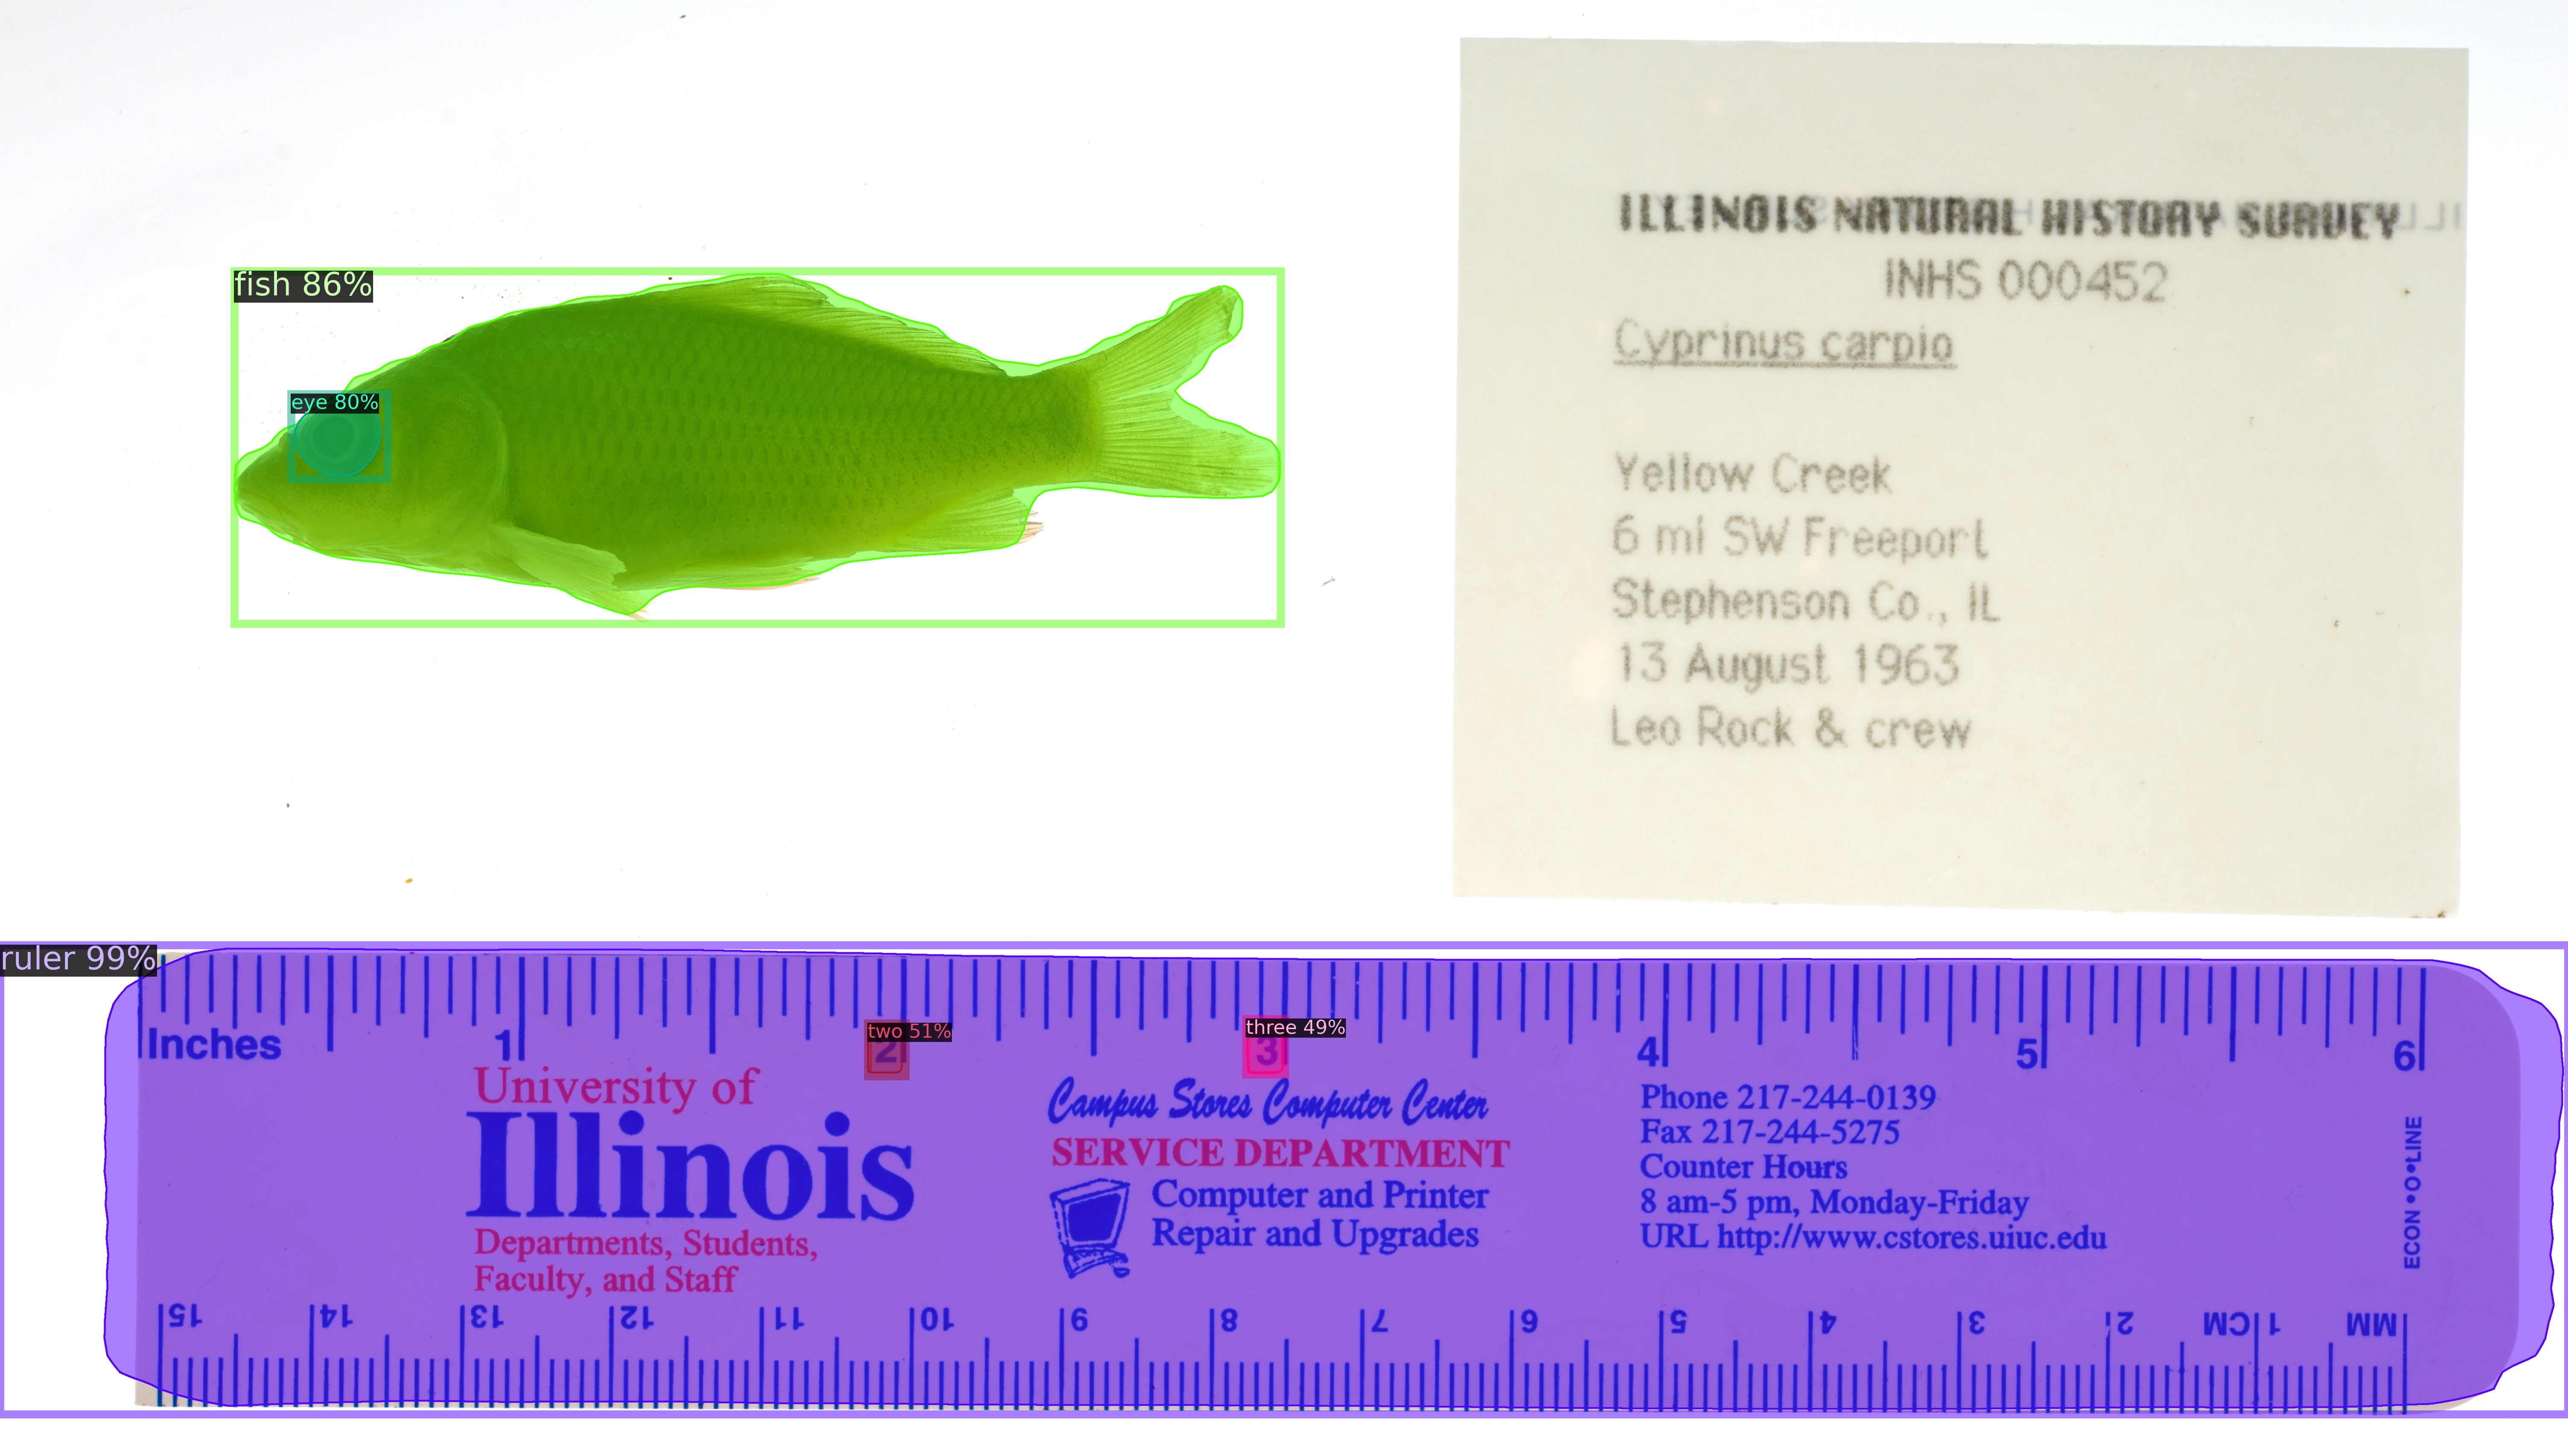
\includegraphics[width=.45\linewidth]{images/teaser1_crop}
  \hspace{5mm}
  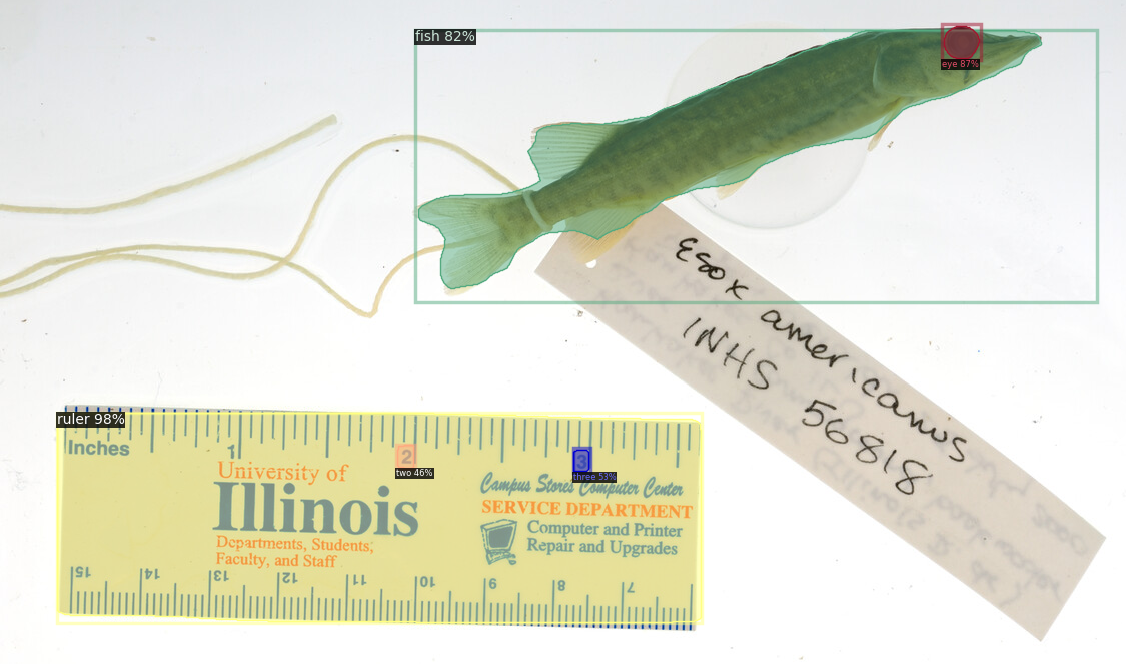
\includegraphics[width=.45\linewidth]{images/teaser2_crop}
  \caption{Initial object detection on two specimen images using Detectron2~\cite{wu2019detectron2}.}
  \label{fig:teaser}
\end{figure*}

3) Compute a number of high-level metadata properties from the detected objects and image quality metrics.
% [*Test our ability to calculate] the following set of
% : 1) contrast (intensities of the foreground and background, 2) centroid and eye center, and if eye is found, the fish 3) side 4) primary axis and clock value, finally the 5) scale and length.

4) Compare computed metadata properties with manually generated properties
when possible to assess the accuracy and effectiveness of automated 
methods.

%Following is original Goals/objectives text: The amount of data is immense, with image collections containing 10,000's of entries. These discoveries will only be possible with computational techniques that can process this vast amount of data.

%These image-based computational techniques are hampered by both poor image quality and the lack of high-quality and pertinent metadata associated with collections.

%For example, a study may require images that contain only one fish with a given level of lighting and contrast. Additionally, performing quantitative investiations into the morphology of the specimens requires knowing the physical scale of the images, i.e.~pixels/inch.

%Given the many thousands of images that have and will be acquired of biological specimens, it is infeasible to generate the needed metadata via manual, i.e. via human input, methods.  It is critical to deploy computational techniques that will automate the process of generating the metatdata that is essential for downstream analyses and studies.

%In order to address the need for fish specimen image metadata that can support scientific investigations we have begun the deployment of both off-the-shelf and custom-written software that automatically generates a variety of metadata from a publicly-available biological image repository.  The types of metadata being produced are related to image quality, content and scale, and should provide the information necessary for advanced quantitative studies of the digitized specimens.

The automated metadata generation methods for our project were developed to work on a specific set of images, the INHS\ Fish Collection~\cite{INHS}.  Most of these images have been configured, produced and acquired with a standard procedure.  The images used for our study contain one fish placed on a bright, white background and contain an information tag and the same ruler.  See Figure \ref{fig:INHS_examples} for three example images from the collection. While training and focusing our system on images with very similar compositions and visual properties may limit its immediate applicability, our efforts demonstrate the potential that machine learning and image informatics techniques have for automatically generating metadata for biological specimen image collections in general.

\section{Methods}
Our process for metadata generation can be broken into three steps: 1) object detection with Facebook's Detectron2 machine learning library (subsequently referred to as \verb|detectron|), 2) image processing at the pixel level, and 3) calculations on the results of the previous steps to determine higher level metadata properties.
% \todo{Definitely need to explain somewhere in more detail about our current admissibility criteria for images. Not sure where I want to put it yet so just leaving it as a todo}

\subsection{Detectron}
A prerequisite task to performing any advanced metadata property generation
is finding the specimens (and other relevant objects) within the collection
images. Object detection has been a broadly active field of study in recent
years \cite{zou2019object}, and has resulted in a number of well-tested, purpose-built architectures. We elected to use Facebook AI Research's (FAIR)
\verb|detectron| tool \cite{wu2019detectron2}, and specifically its implementation of the Mask R-CNN architecture \cite{he2018mask}, for object detection in our project.
\verb|detectron| is built on \verb|pytorch|~\cite{NEURIPS2019_9015} and provides a relatively straightforward method for training on COCO~\cite{DBLP:journals/corr/LinMBHPRDZ14} format datasets. It is able to handle an arbitrary number of object classes, and can classify an arbitrary number of object within a given image. We chose \verb|detectron| for its relative ease of use compared to lower level libraries, and its implementations of powerful architectures developed by FAIR.
For our project, we use it to identify five object classes: fish, fish eyes, rulers, and the numbers 2 and 3 on rulers,
as shown in Figure \ref{fig:teaser}. Objects with a 30\% confidence score or higher are maintained for analysis.

% Not sure wrapping this is really getting us much after the 2 column switch

%\begin{wraptable}{r}{5.5cm}
\begin{table}[H]
    \centering
      \caption{Training dataset}
    \label{tab:dataset}
    \begin{tabular}{cccc}
        \toprule
        \textbf{Class} & \textbf{Number of Instances}\\
        \midrule
        Fish & 297\\
        Ruler & 1496\\
        Eye & 456\\
        Two & 100\\
        Three & 100\\
      \bottomrule
    \end{tabular}
\end{table}
%\end{wraptable}

Table \ref{tab:dataset} lists the number of instances for each class 
used in our training dataset.
All of the training data was labeled by hand using \verb|makesense.ai| \cite{make-sense}
% While the ultimate goal of the project is to generalize to images from a variety of specimen collections, we have thus far focused only
on images from the INHS\ Fish Collection \cite{INHS}.
Using \verb|detectron|'s default training scheme, the model was trained for \(100,000\) epochs. All instance types were included in a single object detection model. The total cross-entropy loss began at \(2.948\) and ended at \(0.158\) for the training data.

\begin{comment}
\begin{verbatim}
|  category  | #instances   |  category  | #instances   |  category  | #instances   |
|:----------:|:-------------|:----------:|:-------------|:----------:|:-------------|
|    fish    | 297          |   ruler    | 1496         |    eye     | 456          |
|    two     | 100          |   three    | 100          |            |              |
|   total    | 2449         |            |              |            |              |

Iterations: 100,000

Initial: {"data_time": 0.004866079999999329, "fast_rcnn/cls_accuracy": 0.115234375,
"fast_rcnn/false_negative": 0.1686291000841043,
"fast_rcnn/fg_cls_accuracy": 0.2782012195121951, "iteration": 5, "loss_box_reg": 0.40475407242774963,
"loss_cls": 1.8559419512748718, "loss_mask": 0.6982034742832184, "loss_rpn_cls": 0.05218731239438057,
"loss_rpn_loc": 0.007734265644103289, "lr": 0.00011990000000000001, "mask_rcnn/accuracy": 0.2920252418802887,
"mask_rcnn/false_negative": 0.9506743610216735, "mask_rcnn/false_positive": 0.2467277275646746,
"roi_head/num_bg_samples": 115.0, "roi_head/num_fg_samples": 13.0, "rpn/num_neg_anchors": 251.25,
"rpn/num_pos_anchors": 4.75, "time": 0.2812129614999961, "total_loss": 2.9480794025585055}

Final: {"data_time": 0.006645713496254757, "eta_seconds": 0.0, "fast_rcnn/cls_accuracy": 0.984375,
"fast_rcnn/false_negative": 0.0, "fast_rcnn/fg_cls_accuracy": 1.0, "iteration": 99999,
"loss_box_reg": 0.054501257836818695, "loss_cls": 0.03908616118133068, "loss_mask": 0.06379510834813118,
"loss_rpn_cls": 0.0010549294238444418, "loss_rpn_loc": 0.005114196799695492, "lr": 0.02,
"mask_rcnn/accuracy": 0.9722937165937804, "mask_rcnn/false_negative": 0.012800597698663846,
"mask_rcnn/false_positive": 0.05609636495338312, "roi_head/num_bg_samples": 115.75,
"roi_head/num_fg_samples": 12.25, "rpn/num_neg_anchors": 246.5, "rpn/num_pos_anchors": 9.5,
"time": 0.3563086399990425, "total_loss": 0.15775199318886735}
\end{verbatim}
\end{comment}
\subsection{Pixel Analysis}
The masks and bounding boxes produced by \verb|detectron| are generally quite good, although they almost never completely or tightly enclose the
detected objects.
This is problematic for the detected fish objects in our analyzed images,
where the most accurate segmentation is desired.
The mask may include additional background as part of the fish, or the
bounding box may clip away part(s) of the fish. To solve these
shortcomings, we utilize pixel analysis methods commonly found in image
informatics to produce more accurate object masks and bounding boxes.

\begin{table*}[t]
    \centering
    \caption{Metadata properties (* indicates higher order derived properties)}
    \label{tab:properties}
    \begin{tabular}{cccp{0.5\linewidth}}
        \toprule
        \textbf{Property} & \textbf{Association} & \textbf{Type} & \textbf{Explanation}\\
        \midrule
        \verb|has_fish| & Overall Image & Boolean & Whether a fish was found in the image.\\
        \verb|fish_count| & Overall Image & Integer & The quantity of fish present.\\
        \verb|has_ruler| & Overall Image & Boolean & Whether a ruler was found in the image.\\
        \verb|ruler_bbox| & Overall Image & 4 Tuple & The bounding box of the ruler (if found).\\
        \verb|scale|* & Overall Image & Float & The scale of the image in \(\frac{\mathrm{pixels}}{\mathrm{cm}}\).\\
        \verb|bbox| & Per Fish & 4 Tuple & The top left and bottom right coordinates of the bounding box for a fish.\\
        \verb|background.mean| & Per Fish & Float & The mean intensity of the background within a given fish's bounding box.\\
        \verb|background.std| & Per Fish & Float & The standard deviation of the background within a given fish's bounding box.\\
        \verb|foreground.mean| & Per Fish & Float & The mean intensity of the foreground within a given fish's bounding box.\\
        \verb|foreground.std| & Per Fish & Float & The standard deviation of the foreground within a given fish's bounding box.\\
        \verb|contrast|* & Per Fish & Float & The contrast between foreground and background intensities within a given fish's bounding box.\\
        \verb|centroid| & Per Fish & 4 Tuple & The centroid of a given fish's bitmask.\\
        \verb|primary_axis|* & Per Fish & 2D Vector & The unit length primary axis (eigenvector) for the bitmask of a given fish.\\
        \verb|clock_value|* & Per Fish & Integer & Fish's primary axis converted into an integer ``clock value'' between 1 and 12.\\
        \verb|length|* & Per Fish & Float & The length of a fish in \(\frac{\mathrm{pixels}}{\mathrm{cm}}\).\\
        \verb|mask| & Per Fish & 2D Matrix & The bitmask of a fish in 0's and 1's.\\
        \verb|pixel_analysis_failed| & Per Fish & Boolean & Whether the pixel analysis process failed for a given fish. If \verb|true|, \verb|detectron|'s mask and bounding box were used for metadata generation.\\
        \verb|score| & Per Fish & Float & The percent confidence score output by \verb|detectron| for a given fish.\\
        \verb|has_eye| & Per Fish & Boolean & Whether an eye was found for a given fish.\\
        \verb|eye_center| & Per Fish & 2 Tuple & The centroid of a fish's eye.\\
        \verb|side|* & Per Fish & String & The side (i.e.\ \verb|'left'| or \verb|'right'|) of the fish that is facing the camera (dependent on finding its eye).\\
      \bottomrule
\end{tabular}
\end{table*}

\subsubsection{Threshold Adjustment}
The first calculation in the pixel analysis process determines the cutoff intensity between what constitutes the foreground (i.e.~the fish) and background of the image.
Initially, the calculation is based on the bounding box and mask generated by
\verb|detectron|. Specimen images are read in as gray scale, and pixels in the image are treated as unsigned integers between 0 and 255.
Otsu thresholding \cite{Otsu1979ATS}, a technique that maximizes the variance between the 
foreground and background intensities, is used to compute an initial cutoff value between foreground and background. 
While the Otsu value occasionally generates an accurate mask as is, usually
the contrast between foreground and background is low and much of the lighter parts of the fish (such as its tail fin) are marked as background.

To overcome this under-segmentation, the threshold value should be
either adjusted up or down, depending on if the background is lighter or darker than the fish.
For our current dataset, the background is always lighter (i.e.~closer to 255), so the threshold value needs to be scaled up to include more of the
foreground image.
% Precisely how much to scale this value by is difficult to determine.
For optimal results the scaling should be dependent on the
contrast between the background and foreground,
which can be affected by
% both how washed out the image is and
the level of pigmentation of the fish.
% To take this into account, we compute the mean intensity of the foreground and background pixels, then use these intensity values and the difference between them to scale the threshold value.
% Even with these values in hand it is not entirely clear how to scale the threshold.
We found that an improved threshold value can be computed as the halfway
point between the Otsu threshold value and the
mean of the background intensities.
This adjusted threshold value
% by 50\% of the difference between the mean of the background and the original threshold value, which 
struck a fairly optimal balance between capturing most of fish's fins in most cases, without also masking parts of the background.

\subsubsection{Consolidating the Foreground}
While thresholding has the potential to generate better masks than a neural network (when provided an initial approximate bounding box), it also introduces considerable noise. Single or small groups of errant pixels can be marked as foreground depending on the consistency of the background, and interior pixels of the fish (especially around the fins) can be marked as background. To be useful for generating an accurate bounding box and for subsequent computational analysis, the mask must consist of one single ``blob'' over the fish the contains no holes, and no other pixels disconnected from this blob can be marked as foreground.

To accomplish this, we apply an iterative process of flood filling from all the foreground pixels in the image until a blob is generated that is large enough to constitute the fish. This is another metaparameter, but greater than 10\% of the current bounding box has masked the specimen in all observed cases. Once the fish's blob is found, noise then needs removed. This is done by flood filling from each of the corner of the bounding box where the specimen is not present (all four corners in the overwhelming majority of cases), then taking the inverse of the result. The fish mask is excluded from these corner flood fills, so this process removes all noise from both the background and foreground of the image leaving only a close mask over the fish itself.

\subsubsection{Adjusting the Bounding Box}
With an accurate mask generated, it is then necessary to check whether the bounding box needs expanded or shrunk along any edges. Expansion is done first, by checking whether any edge intersects with any of the foreground mask pixels. If one does, it is expanded out by 1 pixel. If any edges are expanded, the whole process of masking and expansion process is repeated to account for any changes in average intensities. Once no edges contain foreground pixels, the mask is then shrunk. This process is more efficient as all that is required is to shrink each edge by one up until the point they contain one or more foreground pixels. Once the shrinkage step is accomplished, the final mask and bounding box have been generated.

\subsubsection{Fallback} The pixel analysis process occasionally fails,
e.g.\ when flood-filling does not produce a large enough blob or
the bounding box adjustment does not terminate.
This can occur if certain flood fill operations behave unexpectedly, or if the image is too washed out or otherwise atypical for the thresholding process to work correctly. In the event this happens, the original mask and bounding box generated by \verb|detectron| is used for metadata generation.

\subsection{Metadata Generation}

The following metadata properties are generated from the methods
described above:
\verb|has_fish|, \verb|fish_count|, \verb|has_ruler|, \verb|ruler_bbox|, \verb|background.{mean,std}|, \verb|foreground.{mean,std}|, \verb|bbox|, \verb|mask|, \verb|score|, and \verb|has_eye|.
The remaining properties are computed as described below, with all the
metadata properties listed in Table \ref{tab:properties}.

\subsubsection{contrast}
The contrast between the intensities of the foreground and background
pixels is computed as \verb|background.mean| - \verb|foreground.mean|.

\subsubsection{centroid and eye\_center}
Centroids are provided for the masks and bounding boxes generated by \verb|detectron|, and since we do not recalculate the mask of fish eyes we can use that value directly for \verb|eye_center|.

Since we recalculate the mask of the fish, its centroid must be recalculated
as well. This can be done via
\begin{equation}
    (\bar{x}, \bar{y}) = (\mathrm{round}(\frac{M_{10}}{M_{00}}), \mathrm{round}(\frac{M_{01}}{M_{00}})),
\end{equation}
where \(M_{00}\) is the pixel area of the fish's blob, \(M_{10}\) is the sum of all the \(x\) values of blob pixels, and \(M_{01}\) is the sum of all the \(y\) values of blob pixels.
\subsubsection{side}
Determining which \verb|side| of the fish is visible is predicated on finding its eye. If an eye is found, the sign of the \(x\) component of the vector from the centroid of the fish to the centroid of the eye specifies which side is up: negative for left and positive for right. This assumes the fish was photographed vertically (i.e.\ dorsal fin on top), which is essentially always the case for all image collections our group has worked on.
\subsubsection{primary\_axis and clock\_value}
The \verb|primary_axis| of a fish can be calculated by taking the covariance of its blob in \(x\) and \(y\), which yields its principle eigenvector.
The eigenvector can be directly assigned to the property. If an eye is
present, we ensure that \verb|primary_axis| points in the direction of the
eye in relation to the fish's centroid.

Our team encoded this information as a ``clock value'' between 1 and 12 when manually recording it. To convert \verb|principal_axis| to \verb|clock_value|, the sign of \(x\) and \(y\) on the principal axis are used to determine which Cartesian quadrant the fish angles into relative to its centroid. 
Depending on this quadrant, we dot product the principal axis with either \([-1,0]\), \([0,-1]\), \([1,0]\) or \([0,1]\), which correspond to 9, 6, 3 and ``0'' o'clock respectively. The resulting radian value is then converted to a polar displacement in clock value space, and added to the comparative clock value used in the dot product. This gives the fish's clock value from
0 to \(11.\overline{9}\). Before recording \verb|clock_value| in the output,
the value is rounded to the nearest integer, with a 0 final result replaced with 12.
\subsubsection{scale and length}
\(\frac{\mathrm{pixels}}{\mathrm{inch}}\) can be calculated by measuring the distance in pixels between the digits 2 and 3 (a 1 inch separation) found on the ruler by \verb|detectron|. Converting this to \(\frac{\mathrm{pixels}}{\mathrm{cm}}\) gives the \verb|scale| metadata property as reported in the output.

For the fish \verb|length| property, it is necessary to determine the furthest points from the centroid of the fish in each direction along its major
axis. Since fish are normally measured in a straight line from their snout down the middle of their trunk, every pixel of the fish blob is projected
onto the fish's major axis (as a line through its centroid).
The projection is done by finding the closest point on the
centroid--principal axis line from the pixel's location.
% intersecting the line through the point along the tangent of the principal axis and the aforementioned centroid--principal axis line.
After processing every pixel in the fish blob, computing the distance
between the two furthest projected points gives the length of the fish in pixels. Multiplying this distance by \verb|scale| gives the fish \verb|length| in centimeters.
\begin{comment}
\subsection{Consideration}
Just gonna throw some caveats in here, might be its own section might not
\begin{itemize}
    \item Program falls back to using detectron mask and bbox for metadata generation in the event the mask generation/pixel analysis fails. Failure is defined as never finding a cohesive flood filled mask that covers more than 10\% of the detectron bbox initially. Can provide a statistic on how often this occurs.
\end{itemize}
\end{comment}
\section{Results and Discussion}
Technicians employed by our team have manually generated the 22 metadata properties deemed crucial to the overall BGNN project~\cite{leipzig2021biodiversity} for a large number of INHS images. \(20,699\) total entries were created by 13 technicians that spanned \(8,398\) unique images. Of these \(8,398\) images, \(7,244\) were both not part of the \verb|detectron| training set and met our current admissibility criteria for \verb|detectron| and pixel processing. We ran the metadata extraction program on these \(7,244\) images.
For the properties of image scale, fish length, and fish bounding boxes
(properties not manually generated),
a random sample of 50 specimens from the set of \(7,244\) were analyzed by
hand for comparison.

Our automated process currently generates 6 of the 22 core metadata properties: \verb|if_fish| (\verb|has_fish|), \verb|fish_number| (\verb|fish_count|), \verb|if_ruler| (\verb|has_ruler|), \verb|specimen_angled| (\verb|clock_value|), \verb|specimen_view| (\verb|side|), and \verb|brightness| (\verb|foreground.mean|).
% and \verb|if_background_uniform| (\verb|background.std|).
In addition, our process also calculates contrast, bounding boxes and
fish lengths in centimeters.

\begin{figure}[t]
  \centering
  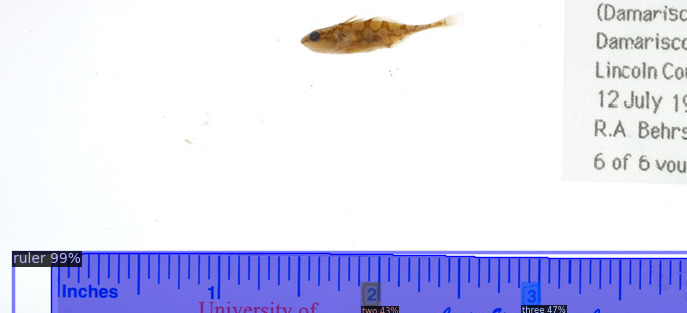
\includegraphics[width=0.9\linewidth]{images/none1_crop} \\
  \vspace{3mm}
  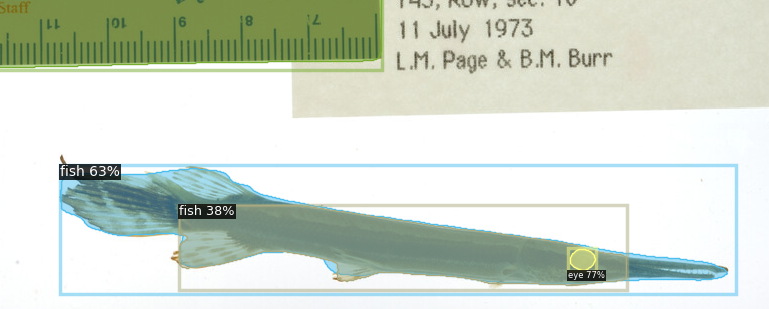
\includegraphics[width=0.9\linewidth]{images/double1_crop}
  \caption{A fish that was not detected (top) and a fish that was detected twice (bottom).}
  \label{fig:fish_detect_wrong}
\end{figure}

\subsection{Fish Detection}
All images in the INHS dataset contain exactly one fish. For \(7,209\) of the specimen images, one fish was detected, a 99.5\% correct rate.
For 25 of the images, 2 fish were detected, 3 fish were detected for 3 images, and for 7 images no fish were found.
The 7 fish that were not detected were quite small. This type of specimen 
is currently lacking from the training set.
See the top image in Figure~\ref{fig:fish_detect_wrong} for an example.
In the case of greater than 1 fish, 9 of the 28 contained tags that
overlapped the fish and were themselves labeled as a second fish.
Of the remaining 17, \verb|detectron| erroneously labeled the fish as two separate fish objects, or labeled a subsection of the fish a second time.
Fish that were double labeled were generally quite large and/or dissimilar from the fish found in the training set, such as the bottom image in
Figure~\ref{fig:fish_detect_wrong}.

\begin{figure}[H]
  \centering
  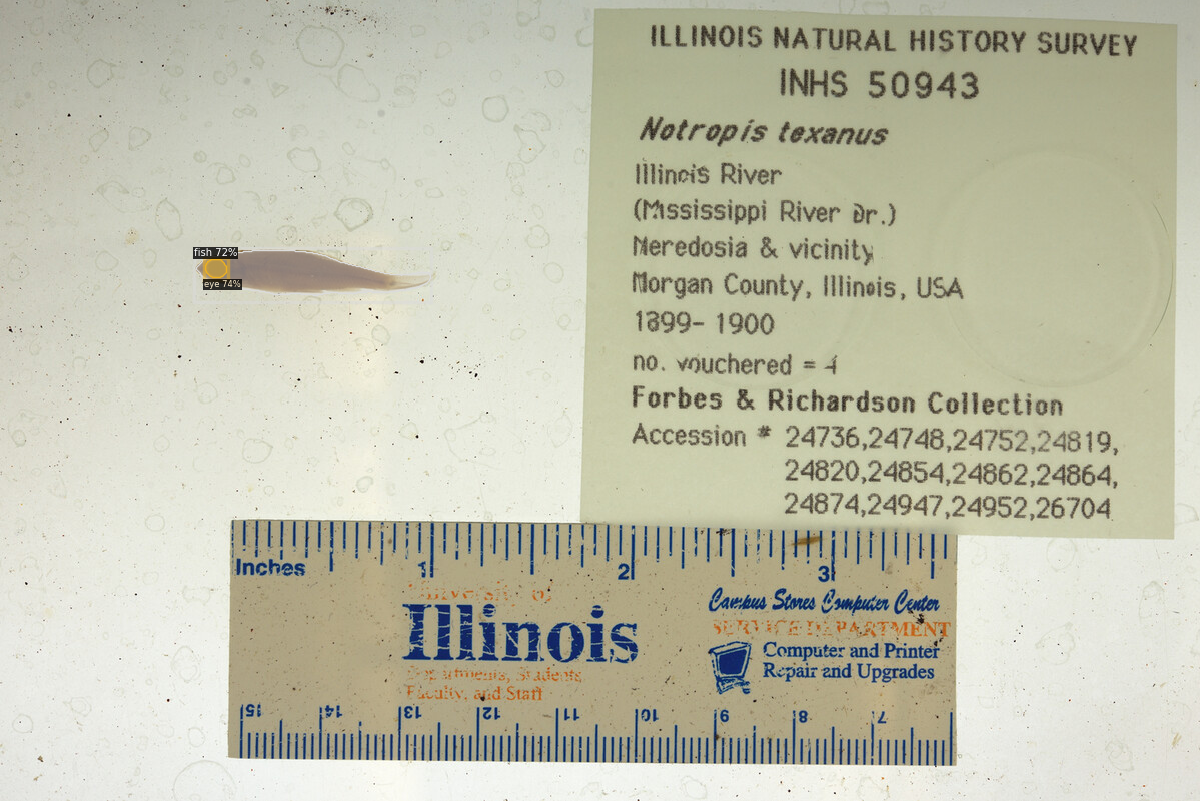
\includegraphics[width=0.49\linewidth]{images/no_ruler1}
  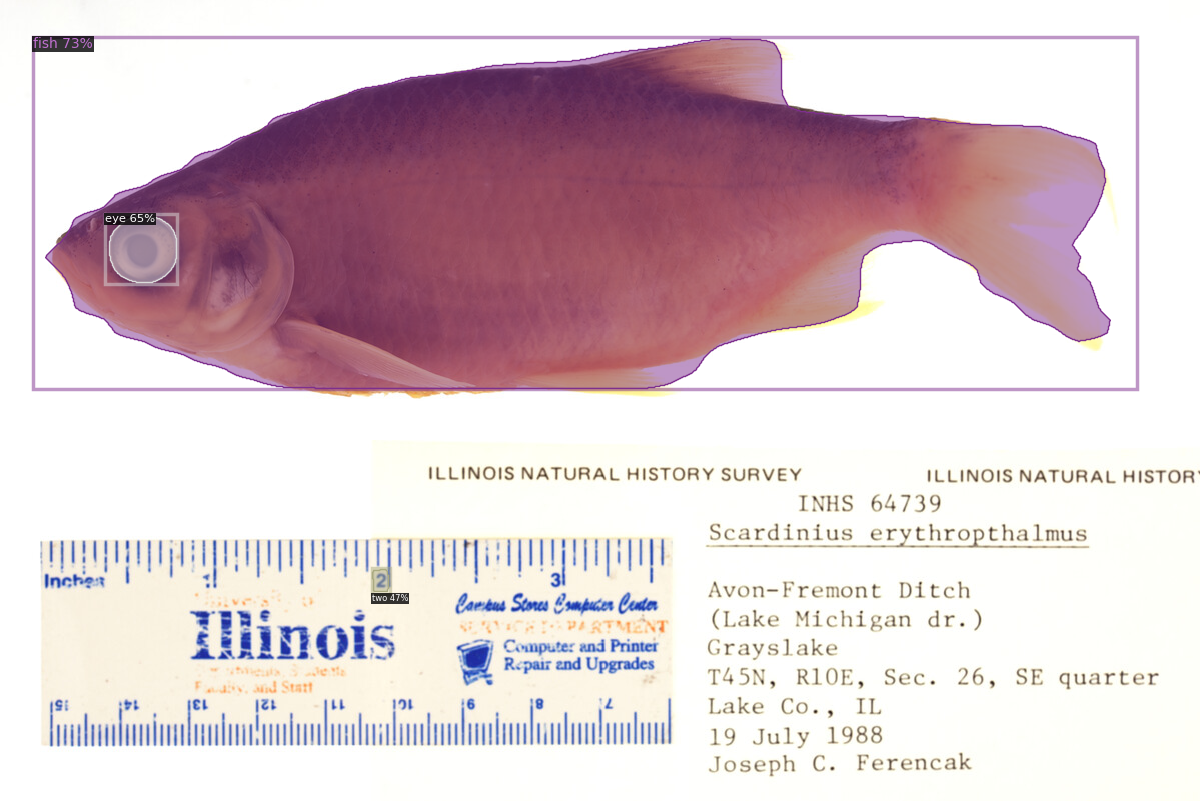
\includegraphics[width=0.49\linewidth]{images/no_ruler2}
  \caption{The two images where the ruler was not found. The left image exhibits a yellow hue, and the right is quite washed out with poor contrast.}
  \label{fig:no_ruler}
\end{figure}


\subsection{Ruler Detection}
For all but 2 of the \(7,244\) images \verb|detectron| was able to find the ruler, a nearly perfect correct rate.
In 56 of the images, the ruler itself was found, but the numbers ``2''
and/or ``3'' on the ruler were not. Therefore, a scale calculation could
not be performed, producing a 99.2\% success rate for
the \verb|scale| computation.

Images where one of these objects were not detected generally had some form of coloration issue. They were either washed out, very dark or yellow in hue.
See Figure \ref{fig:no_ruler} two such examples.
Some of the rulers for which ``2'' and/or ``3'' were not detected were particularly scratched and damaged. Only ``3'' was missed in 45 of the 56 cases, only ``2'' was missed in 2 cases, and both were missed in 9 cases. This may indicate that more training samples for ``3'' are required. Many of the rulers where both numerals were missed were particularly small within the image, which again may be solvable through expanding the training dataset.

%\begin{itemize}
    %\item Worked fairly well all things considered
    %\item Talk about which fish failed
    %\item Talk about which rulers failed
%\end{itemize}

\begin{figure*}[t]
  \centering
  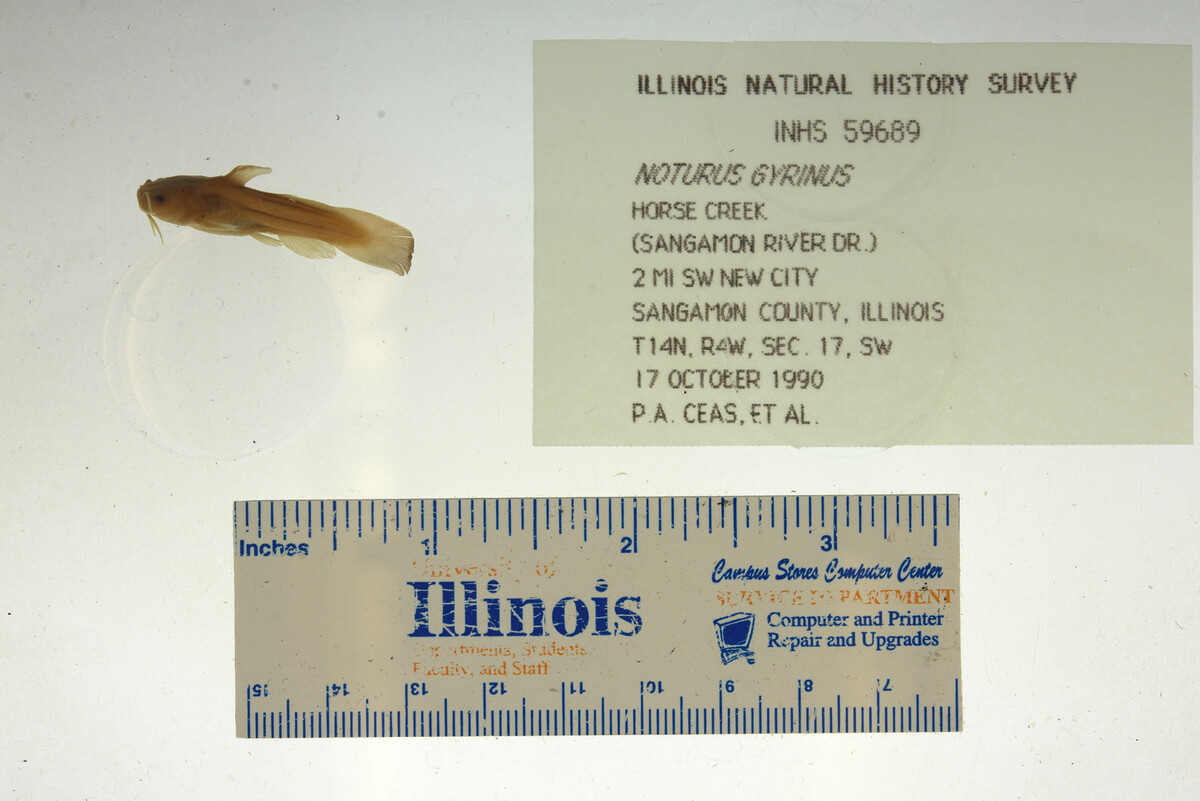
\includegraphics[width=0.31\linewidth]{images/dark}
  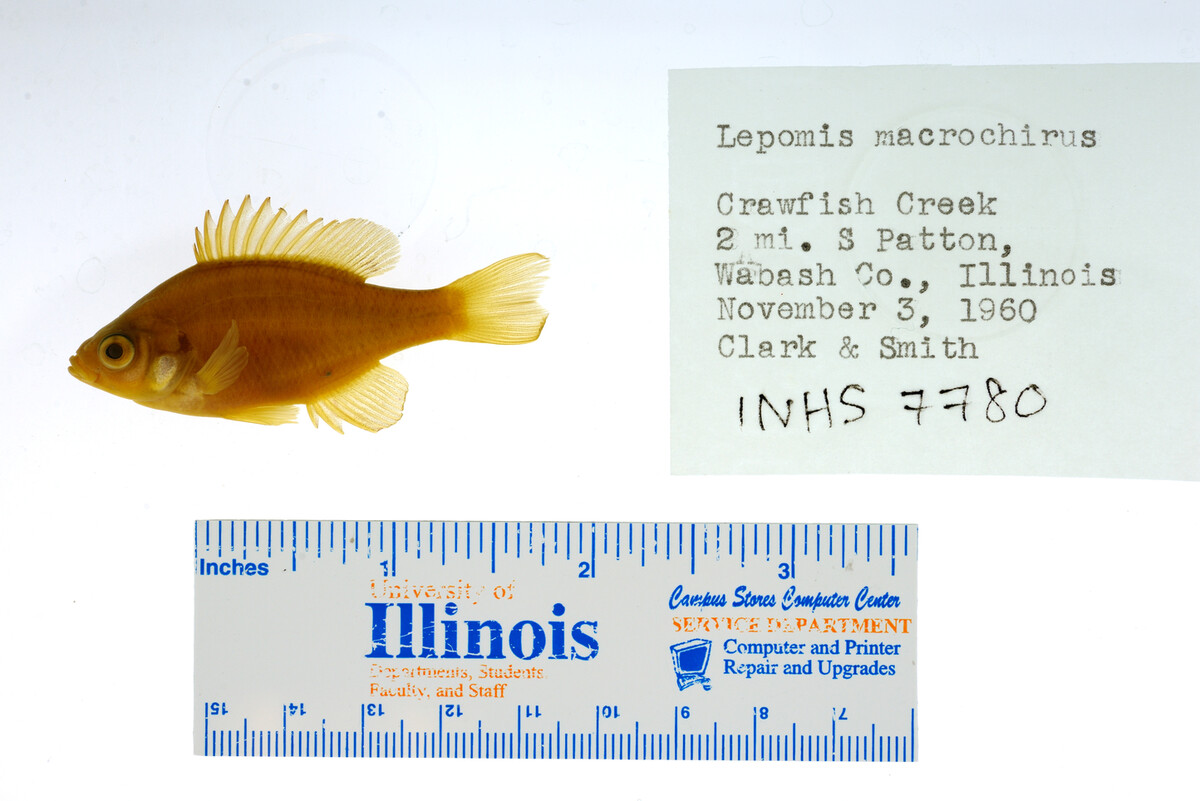
\includegraphics[width=0.31\linewidth]{images/normal}
  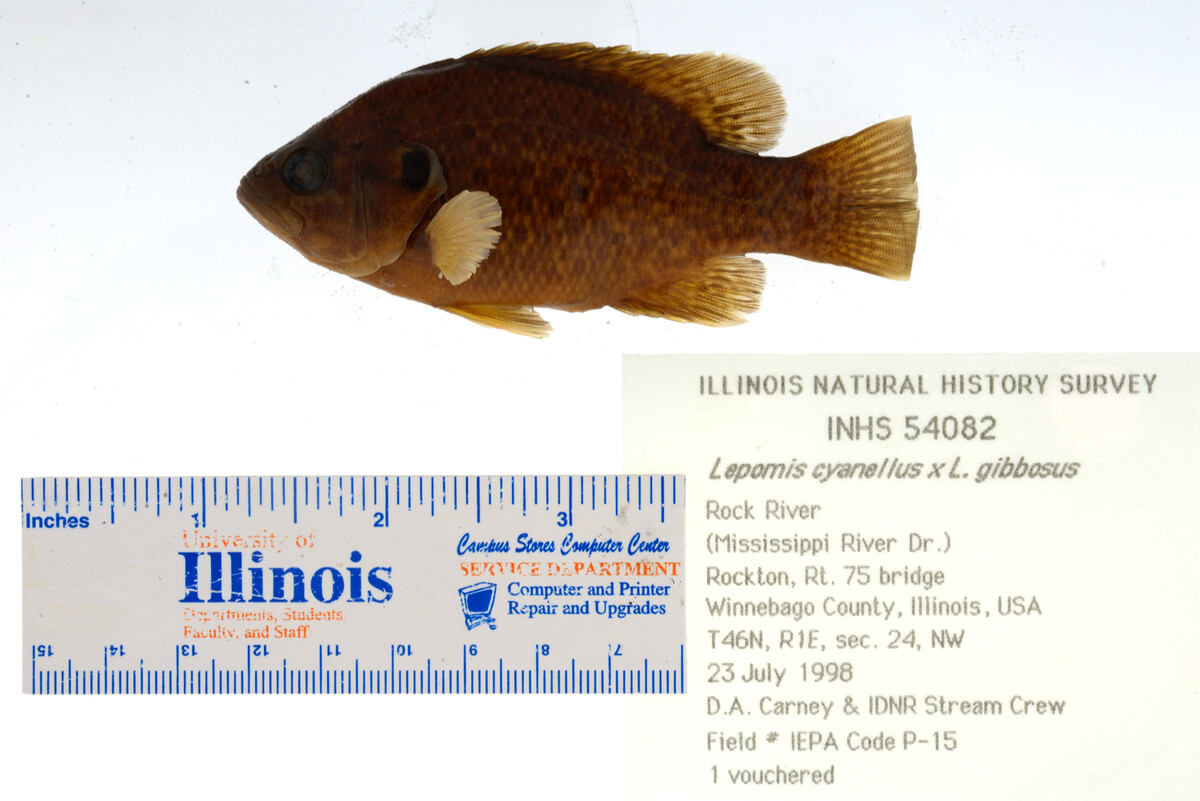
\includegraphics[width=0.31\linewidth]{images/bright}
  \caption{Examples of low, medium and high contrast fish images.}
  \label{fig:contrast}
\end{figure*}

\subsection{Side Detection}
\verb|detectron| was unable to find a fish eye
in 246 of the images. These eyes were generally extremely dark, small, or looked nothing like those found in the training set. Of the remaining \(6,998\) images, the correct side
(\verb|left| or \verb|right|) was detected in all but 6 cases, producing
a 96.5\% correct rate.

% There were six cases where an eye was detected but the \verb|side| value
% was wrong.
For these 6 cases, a spot on the wrong side of the fish was labeled as the
most likely eye within the bounding box of the fish, i.e.\ eye detection 
was incorrect. Figure \ref{fig:wrong_eye} presents one such example.
There were an additional 17 images for which the automated process generated a result that did not match the manually created data. For these remaining cases the manual data was incorrect, giving the automated system an error rate \(2.8\) times lower than the human error rate.
This result highlights the additional utility of automated methods to
double-check and verify human-generated metadata.

\begin{figure}[H]
  \centering
  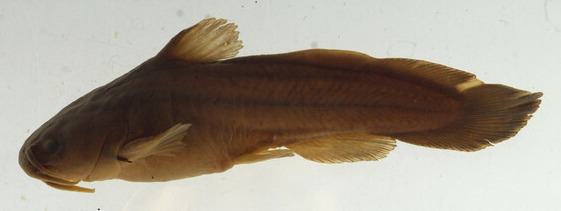
\includegraphics[width=0.49\linewidth]{images/wrong_side_orig}
  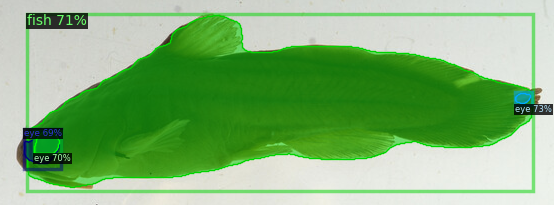
\includegraphics[width=0.49\linewidth]{images/wrong_side1}
  \caption{A fish for which a splotch on its tail fin was labeled the most likely eye.}
  \label{fig:wrong_eye}
\end{figure}

\subsection{Clock Value}
Clock position values were successfully generated for \(6,991\) of the images. Of those, all but 8 were within \(\pm{}1\) of the correct result,
our definition of a correct/acceptable result, making the correct rate for
this computation 96.4\%.

Of the specimens for which clock values were generated, 33 did not match the manually created data (within a tolerance of \(\pm{}1\)).
For 25 of those, the human-generated data was incorrect, giving the automated process a \(3.1\) times lower error rate. Of the 8 that were
computationally classified incorrectly,
two specimens were quite curved making it difficult to assign a clear angle value, as
seen in Figure \ref{fig:curvedFish}.
The other 6 were values of ``3'' instead of ``9'' or vice versa, which resulted from
a mislabeled eye as discussed in the previous section.
%\todo{Why is the following sentence here? What does it have to do with
%Clock Value?}
%A small number of images (such as on the right in Figure~\ref{fig:teaser}) have tags that overlap with the fish. These tags were light enough that they were correctly labeled as background by the pixel analysis.

\begin{figure}[H]
  \centering
  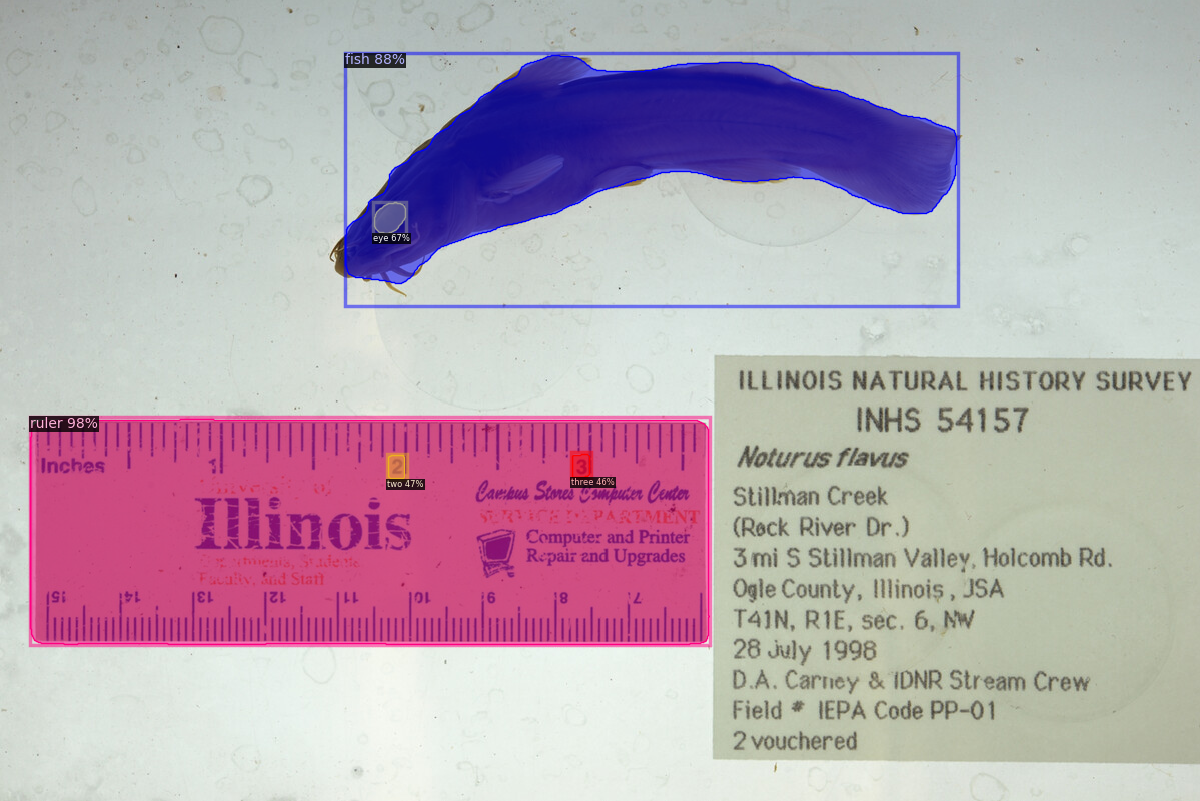
\includegraphics[width=0.7\linewidth]{images/curved1}
  \caption{An example of a heavily curved specimen.}
  \label{fig:curvedFish}
\end{figure}

\begin{comment}
\begin{figure}[t]
  \centering
  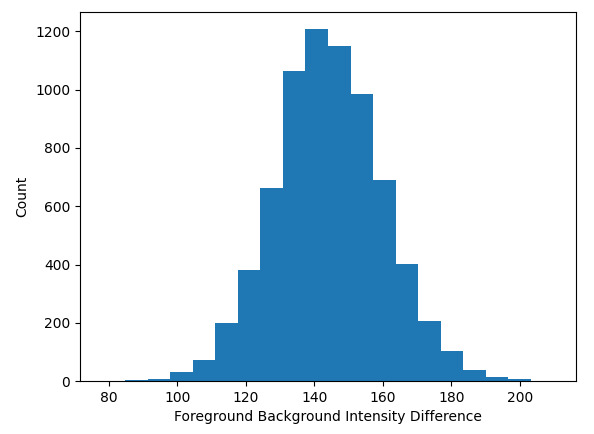
\includegraphics[width=0.9\linewidth]{images/histo}
  \caption{Histogram for difference in brightness between foreground an background.}
  \label{fig:histo}
\end{figure}
\end{comment}

\subsection{Image Contrast}
The contrast of an image is an important image property needed
for the analyses of the BGNN study. Ideally, for INHS images the fish should be well lit and clearly displayed, and the background should also be as light and white as possible.
% Figure~\ref{fig:histo} shows the distribution of
The difference between
the mean intensity of the foreground (i.e.\ the pixels of the fish) and the mean intensity of the background within the fish's bounding box
was computed for all 7,244 images.
The overall mean of the differences is \(144.3\), with a standard deviation of \(15.8\). Images on the low end of the distribution exhibit poor foreground--background contrast, and images on the high end likely contain poorly lit specimens.
Images are considered to have ``low'' and
``high'' contrast if their background-foreground difference is greater than
one standard deviation away from the mean; otherwise they are classified as
``medium''.
Examples of each type of image (low, medium, and high contrast) can be seen in Figure~\ref{fig:contrast}.
The left image has a mean intensity of 103 (low), the middle image 144
(medium), and the right 186 (high).

\begin{table}[H]
    \centering
%    \caption{\verb|foreground.mean| statistics for the three Brightness classes}
    \caption{foreground.mean statistics for the three Brightness classes}
    \label{tab:bright}
    \begin{tabular}{cccc}
        \toprule
        \textbf{Class} & \textbf{Mean Intensity} & \textbf{Standard Deviation} & \textbf{Instances}\\
        \midrule
        Dark & 75.2 & 13.5 & 1800\\
        Normal & 93.6 & 14.8 & 5186\\
        Bright & 108.4 & 15.2 & 242\\
        \bottomrule
    \end{tabular}
\end{table}
\subsection{Brightness}
Specimen brightness is one of the 22 hand-recorded metadata properties. It is encoded as \verb|dark|, \verb|normal| or \verb|bright|. These values
correspond to the mean foreground intensity computed by the automated system.
The mean and standard deviation of the foreground intensities were
computed for the images in the three human-specified classes.
Table~\ref{tab:bright} contains the resulting values and shows that
automated intensities values provide objective measures that may be used to break images into groups that correlate with human-defined brightness
classifications.
The mean of \verb|foreground.mean| over all 7,244 images is 89.5, with a
standard deviation of 16.6. These numbers suggest, for example, that
\verb|foreground.mean| $\pm$ one-half a standard deviation could define 
\verb|normal| brightness, with values outside this range being classified
as \verb|dark| or \verb|bright|.

%\begin{verbatim}
%Standard Deviations for:
    %Uniform: 12.554834863869324
    %Not Uniform: 11.312181711328828
%\end{verbatim}

\subsection{Mask and Bounding Box}

\begin{figure}[t]
  \centering
  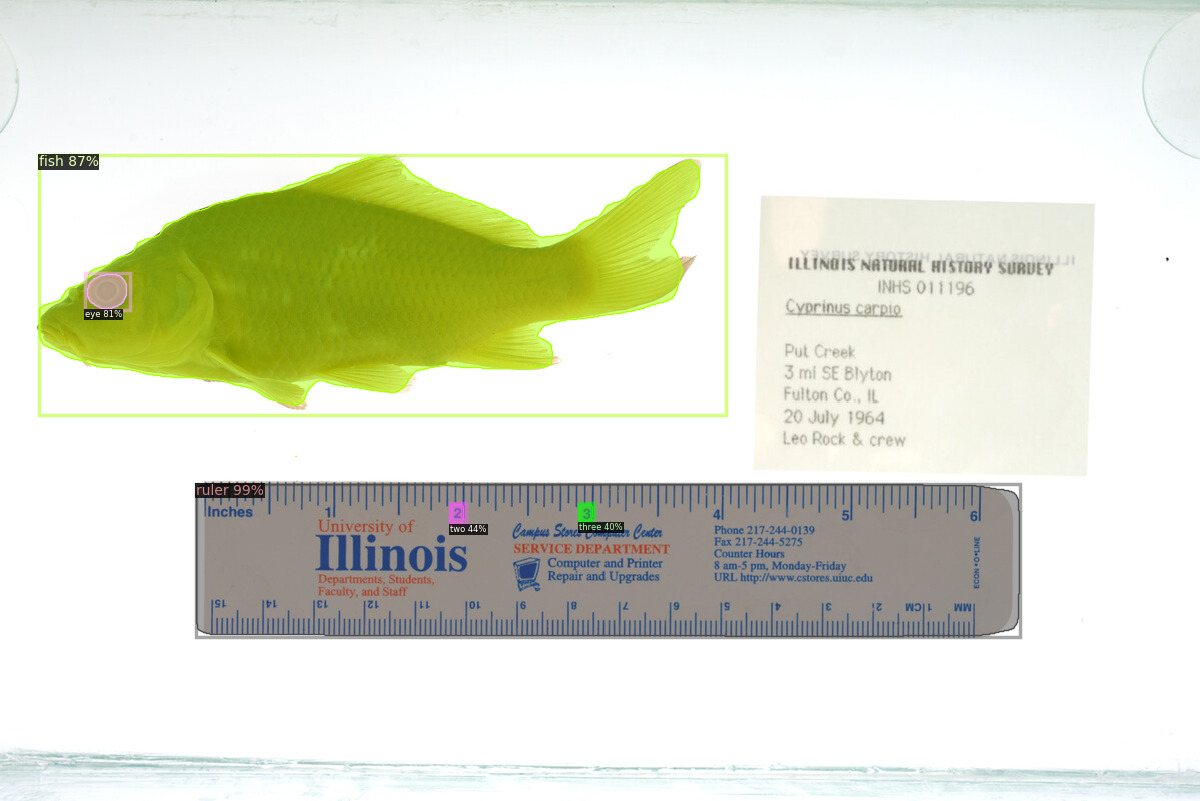
\includegraphics[width=0.49\linewidth]{images/011196_pred}
  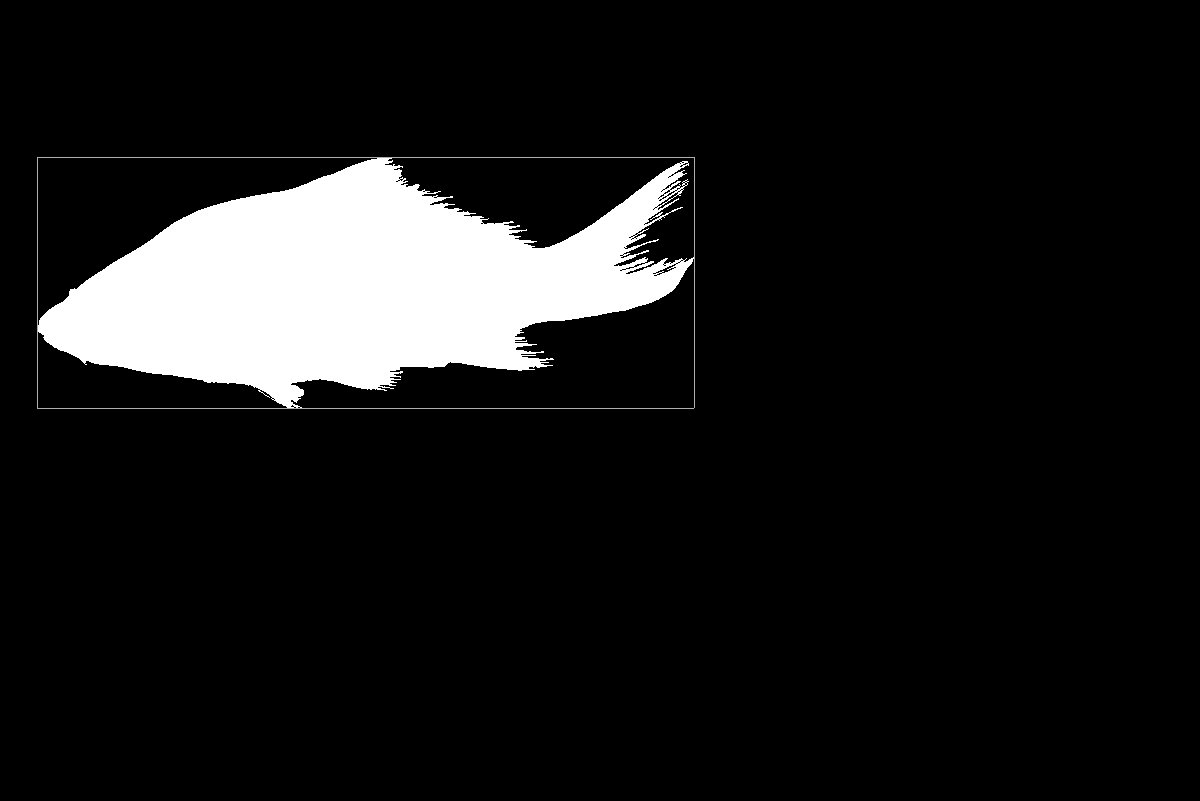
\includegraphics[width=0.49\linewidth]{images/011196_mask}
  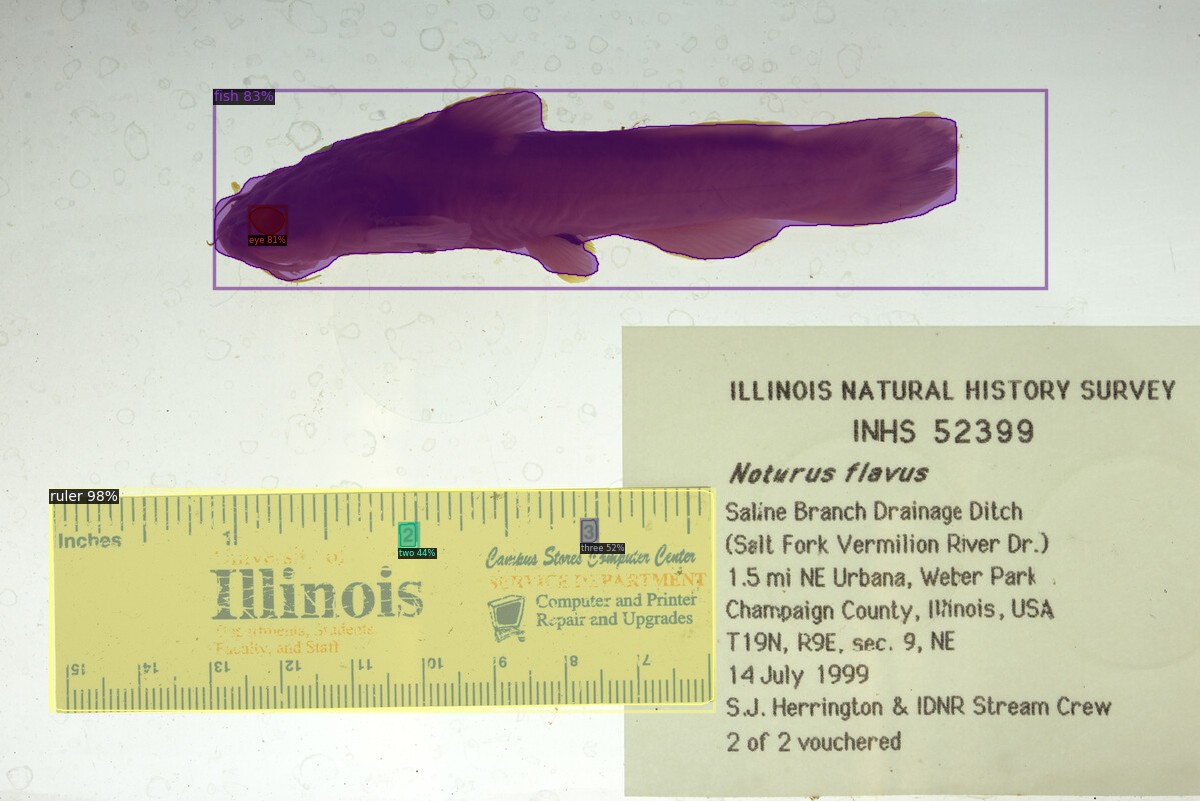
\includegraphics[width=0.49\linewidth]{images/52399_pred}
  
\includegraphics[width=0.49\linewidth]{images/52399_mask}
  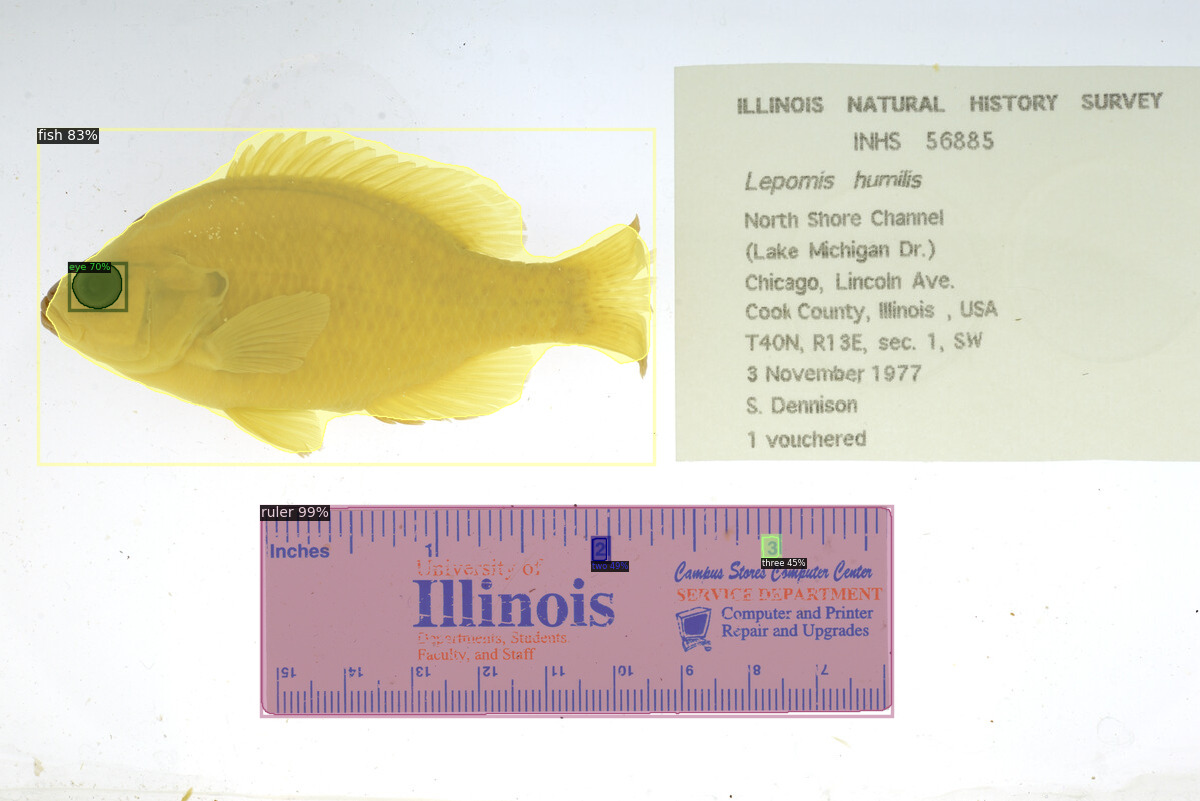
\includegraphics[width=0.49\linewidth]{images/56885_pred}
  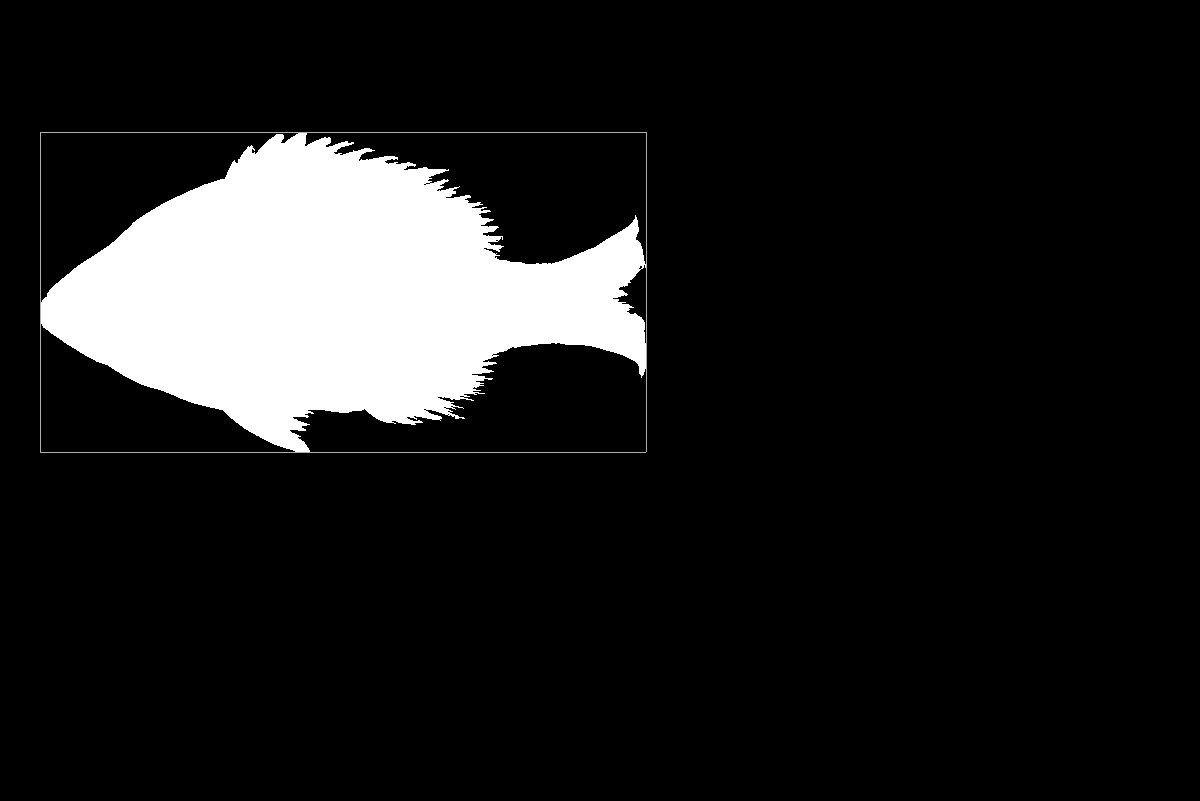
\includegraphics[width=0.49\linewidth]{images/56885_mask}
  \caption{Examples of masks and bounding boxes from detectron (left) and pixel analysis (right).}
  \label{fig:bbox_mask}
\end{figure}

Fish bounding boxes were calculated for all \(7,237\) images in which a fish was found. All but 263 of these were generated via pixel analysis, with those 263 falling back to the original \verb|detectron| bounding box.
50 randomly-chosen images were reviewed manually to evaluate the
calculation, a representative sample are presented in
Figure \ref{fig:bbox_mask}.
All 50 masks and bounding boxes were correctly placed
on/around the location of the fish. However, a number of them lacked portions of lightly colored tails and/or fins.
Specifically, 22 masks and bounding boxes covered the entire fish,
16 missed some of the tail, and 12 missed most or all of the tail, as
seen in Figure \ref{fig:missedTail}.
\begin{figure}[H]
  \centering
  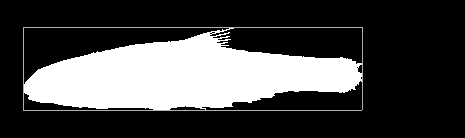
\includegraphics[width=0.49\linewidth]{images/61631}
  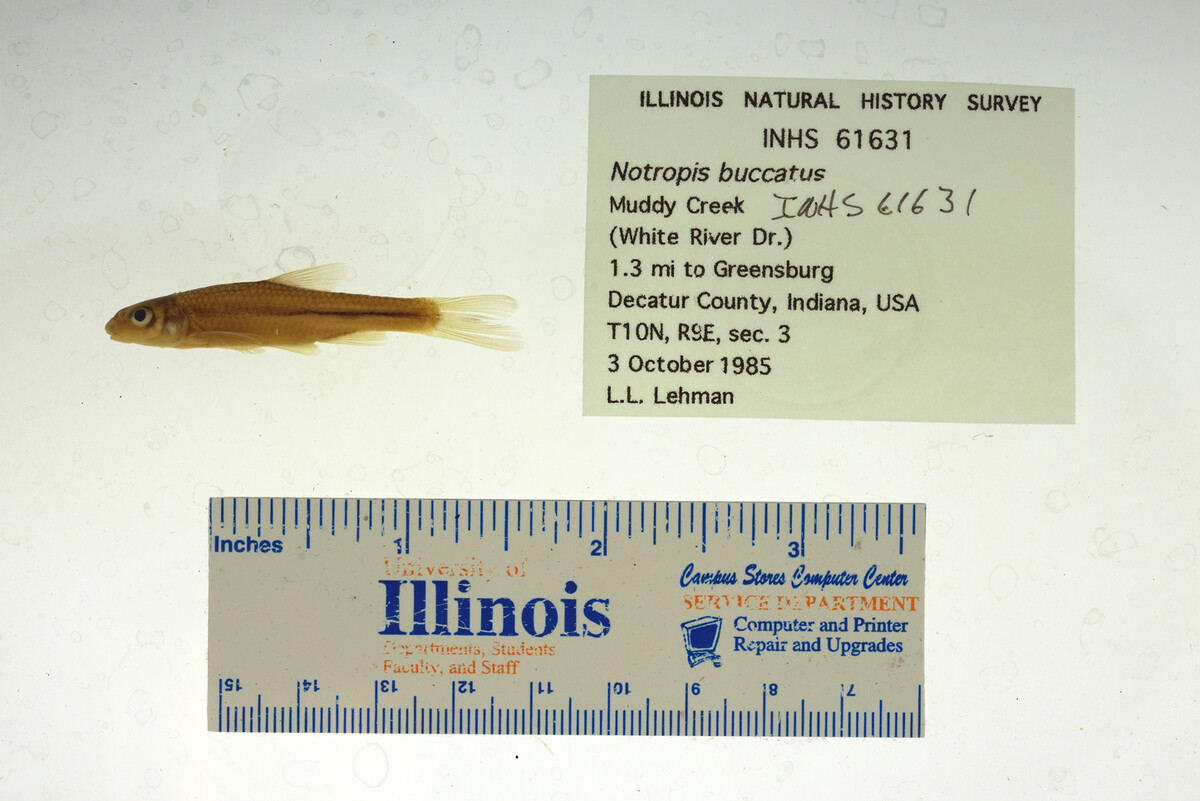
\includegraphics[width=0.49\linewidth]{images/61631_mask}
  \caption{An example of a light colored tail being missed during the pixel analysis process.}
  \label{fig:missedTail}
\end{figure}
Masks and bounding boxes contain the head and trunk of the fish in nearly all cases, but further refinement of our algorithms will be needed
to ensure that light fins and tails are masked consistently and accurately.

\subsection{Scale and Length}
Image scale and fish lengths were calculated for \(7,179\) of the images.
For the remaining 65 images, either the fish, the ``2'' and/or the ``3'' on the ruler were not detected.
Image scale ($\frac{\mathrm{pixels}}{\mathrm{cm}}$) and fish length were
measured, using ImageJ~\cite{imagejCite}, in the same 50 test images.
% 50 of these images \todo{The same 50 as before?} were measured by hand to get \(\frac{\mathrm{pixels}}{\mathrm{cm}}\) and fish length in centimeters with ImageJ~\cite{imagejCite}.
In this subset of images the average error for the scale calculation
was \(0.91\%\), and the average error for the fish length calculation was \(5.87\%\).
Scale calculations using the ``2'' and ``3'' method are nearly identical to those calculated by hand between the tick marks on the ruler. When the tail of the fish is accurately masked and the specimen is fairly straight, the length calculation is highly accurate as well. An example of such a result can be seen in Figure~\ref{fig:scale_len}, for which the difference between the hand measured length and the automatically calculated length was only \(0.6\%\) (\(8.88\) cm vs \(8.82\) cm). Thus, the primary means of lowering the error of the length calculation is to improve tail masking accuracy.
\begin{figure}[H]
  \centering
  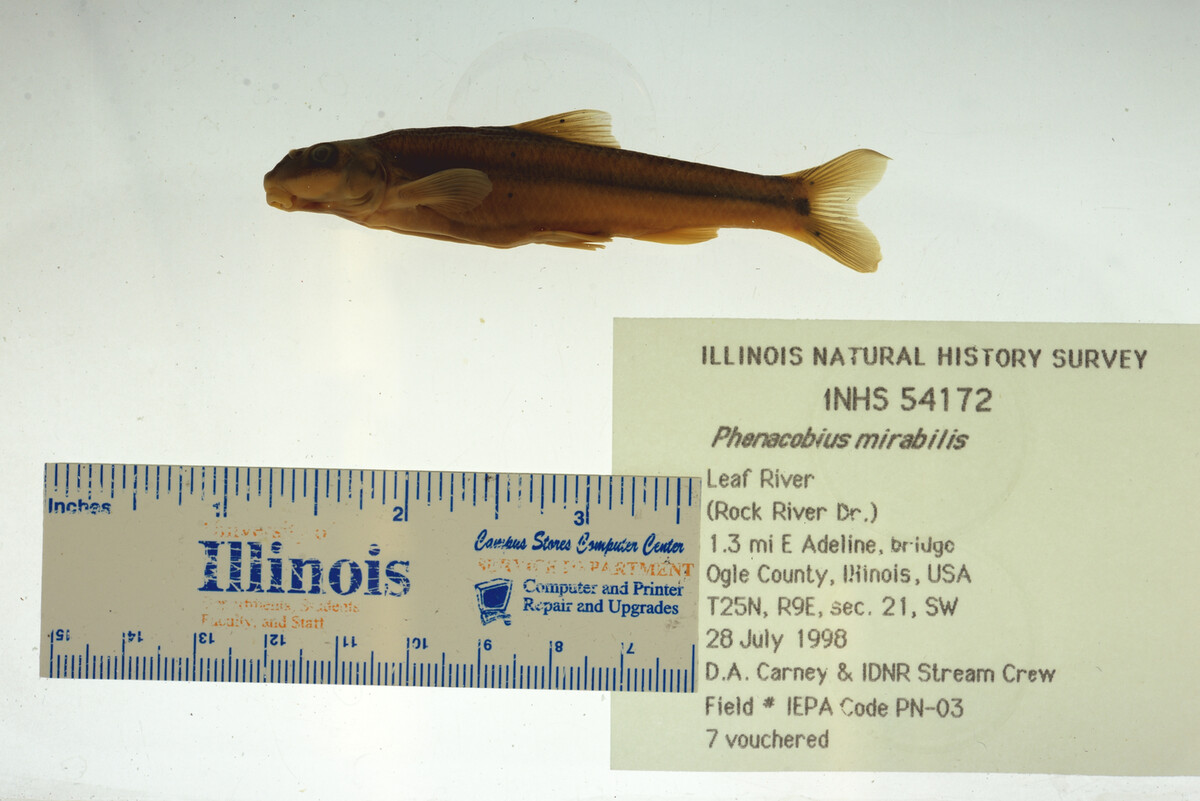
\includegraphics[width=0.49\linewidth]{images/54172}
  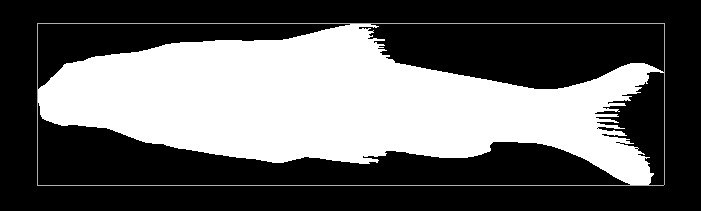
\includegraphics[width=0.49\linewidth]{images/54172_mask}
  \caption{A fish for which the masking and measurement process was highly accurate.}
  \label{fig:scale_len}
\end{figure}

%\section{Discussion}
%\textbf{Todo}: Will need some sort of intro/framing paragraph
%DRAFT from jg: Our results provide insight into how off-the-shelf software, supplemented by additional XXX [programming?] can support automatic metadata generation. Results are promising in a number of respects, helping us to identify more clearly areas, where more work is needed [e.g., failed fish, failed rulers]
%Discussion needed to weave in at least a couple of citations. Happy to discuss
%\begin{figure}[H]
  %\centering
  %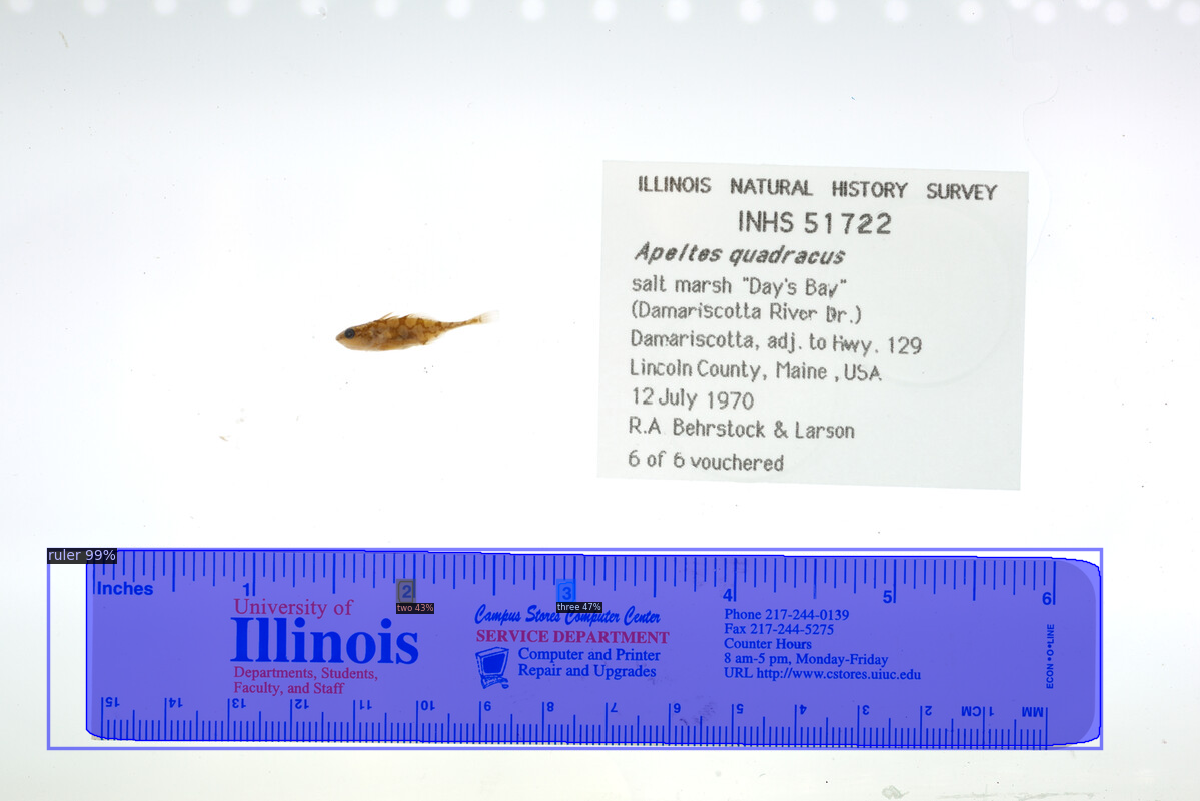
\includegraphics[width=0.49\linewidth]{images/none1}
  %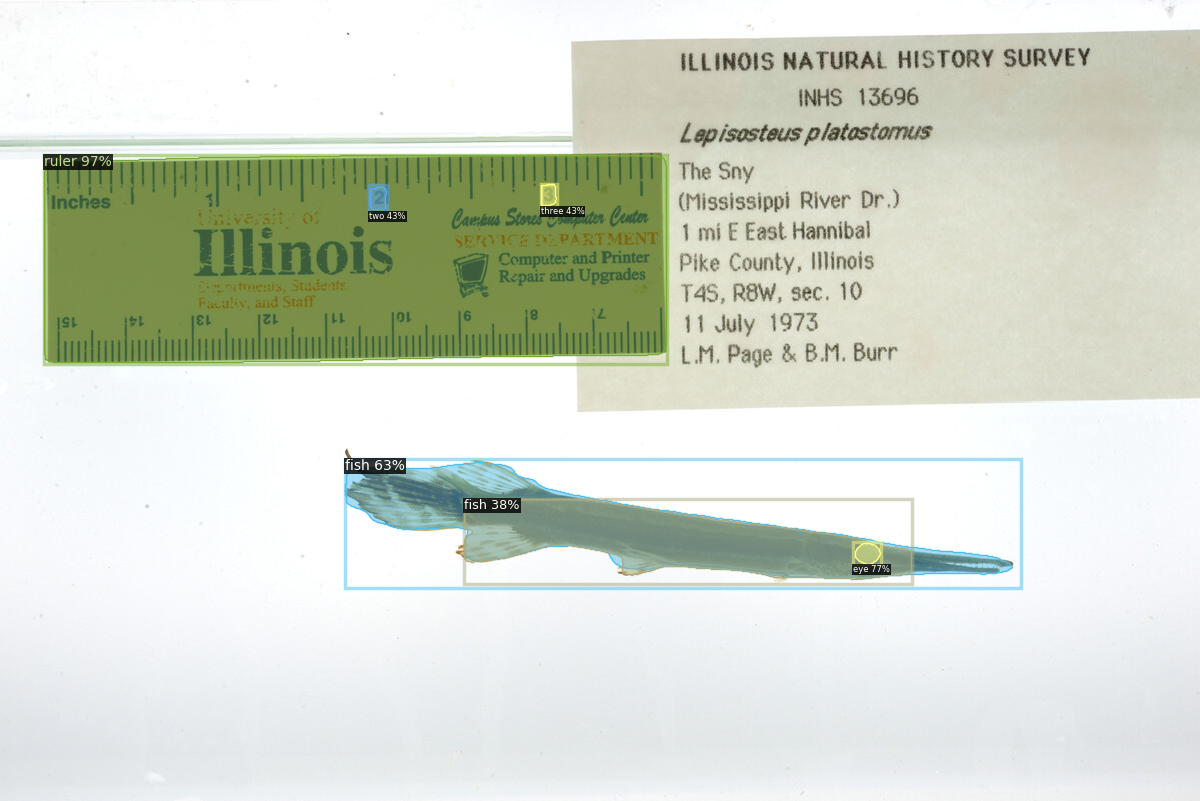
\includegraphics[width=0.49\linewidth]{images/double1}
  %\caption{An example of a fish that was not detected (left) and a fish that was detected twice (right).}
%\end{figure}
%\subsection{Results}\todo{Just going to put the results discussion in small sections and we can change it later if that doesn't make sense}
%\subsubsection{Object Detection}

%\begin{itemize}
    %\item Worked fairly well all things considered
    %\item Talk about which fish failed
    %\item Talk about which rulers failed
%\end{itemize}
%\begin{figure}[H]
  %\centering
  %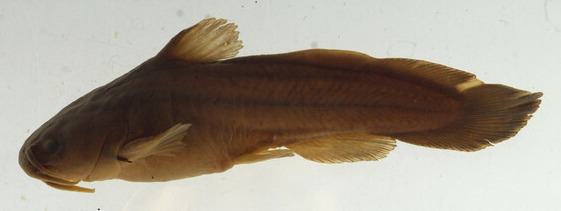
\includegraphics[width=0.49\linewidth]{images/wrong_side_orig}
  %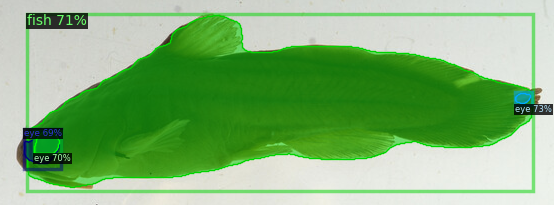
\includegraphics[width=0.49\linewidth]{images/wrong_side1}
  %\caption{A fish for which a splotch on its tail fin was labeled the most likely eye.}
%\end{figure}
%\subsubsection{Side Detection}
%There were six cases where an eye was detected but the \verb|side| value
%was wrong. Here, a spot on the wrong side of the fish was labeled as the
%most likely eye within the bounding box of the fish, i.e.~eye detection 
%was incorrect.
%There were an additional 17 images for which the automated process generated a result that did not match the manually created data. For these remaining cases the manual data was incorrect, giving the automated system an error rate \(2.8\) times lower than the human error rate.
%This result highlights the additional utility of automated methods to
%double-check and verify human-generated metadata.

%\subsubsection{Clock Value}
%\begin{figure}[H]
  %\centering
  %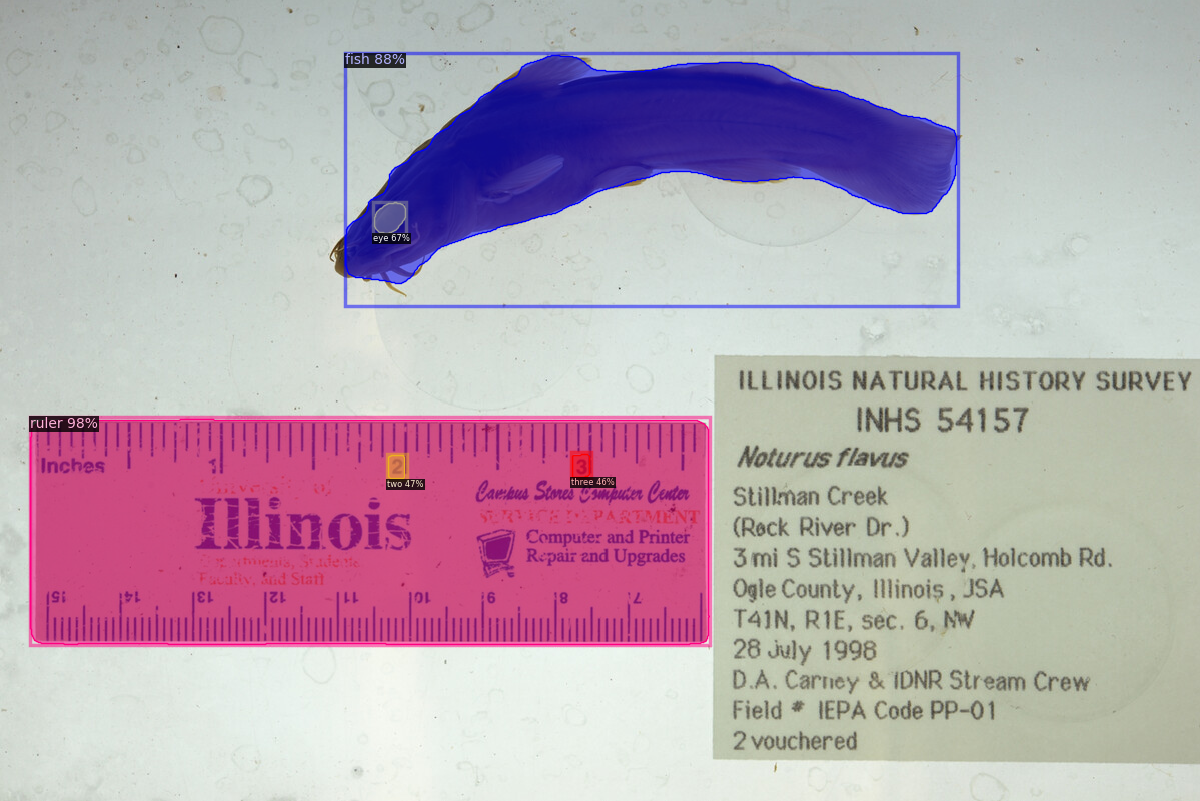
\includegraphics[width=0.49\linewidth]{images/curved1}
  %\caption{An example of a heavily curved specimen.}
  %\label{fig:curvedFish}
%\end{figure}
%Of the specimens for which clock values were generated, 33 did not match the manually created data (within a tolerance of \(\pm{}1\)).
%For 25 of those, the human-generated data was incorrect, giving the automated process a \(3.1\) times lower error rate. Of the remaining 8, 2 specimens were quite curved making it difficult to assign a clear angle value, as
%seen in Figure \ref{fig:curvedFish}.
%The other 6 were values of 3 instead of 9 or vice versa, which resulted from
%a mislabeled eye as discussed in the previous section.
%\todo{Why is the following sentence here? What does it have to do with
%Clock Value?}
%A small number of images (such as on the right in Figure~\ref{fig:teaser}) have tags that overlap with the fish. These tags were light enough that they were correctly labeled as background by the pixel analysis.

%\subsubsection{Mask and Bounding Box}

%\subsection{Scale and Length}
%Image scale and fish lengths were calculated for \(7,179\) of the images.
%\todo{What happened the excluded images?}
%Image scale ($\frac{\mathrm{pixels}}{\mathrm{cm}}$) and fish length were
%measured, using ImageJ~\cite{imagejCite}, in the same(?) 50 test images.
% 50 of these images \todo{The same 50 as before?} were measured by hand to get \(\frac{\mathrm{pixels}}{\mathrm{cm}}\) and fish length in centimeters with ImageJ.~\cite{imagejCite}
%In this subset of images the average error for the scale calculation
%was \(0.91\%\), and the average error for the fish length calculation was \(5.87\%\).


%\section{Discussion}
%\textbf{Todo}: Will need some sort of intro/framing paragraph
%DRAFT from jg: Our results provide insight into how off-the-shelf software, supplemented by additional XXX [programming?] can support automatic metadata generation. Results are promising in a number of respects, helping us to identify more clearly areas, where more work is needed [e.g., failed fish, failed rulers]
%Discussion needed to weave in at least a couple of citations. Happy to discuss

%\subsection{Results}\todo{Just going to put the results discussion in small sections and we can change it later if that doesn't make sense}

%\subsubsection{Brightness?}
%\textit{Like I said in slack, the standard deviation of background does not currently correlate with the is\_background\_uniform property. Brightness results are are in previous section. Need to think about what is worth noting since it's a fairly trivial result.}

\section{Conclusions}
The BGNN project demonstrates a clear need for improved metadata for specimen image collections. Much effort, time and money have been put into photographing and digitizing physical specimen, but without detailed and complete metadata properties the utility of these repositories for advanced computation analysis and machine learning is limited. Since it is prohibitively time intensive to generate all the pertinent properties by hand, automated techniques are needed to generate this missing metadata at scale.

In this paper we presented such a metadata generation program. It produces 6 of the 22 core BGNN metadata properties~\cite{leipzig2021biodiversity}, as well as image contrast, bounding boxes and scale and length information. Testing this program on \(7,244\) images from the INHS dataset~\cite{INHS}, we see that the vast majority of the resulting metadata is correct within a tolerance of a few percentage points, and in some cases contains fewer mistakes than the manually generated validation metadata. Through further refinement and generalizing beyond only INHS images, we aim to create a tool that can be distributed to specimen image collection curators to correct the metadata sparsity that precipitated this work.
\subsection{Future Work}
The most pressing next step is to refine the pixel analysis thresholding process so that the entirety of even light colored fish are marked as foreground in the mask. A deficiency of the current process is that it only operates on single channel intensity. Some of the lightest tails appear yellow in hue to the human eye and easily distinguishable, but when compressed to a single intensity value they are almost identical in value to the white background. Considering when the RGB channels of a pixel are not equal in value may be able to improve masking of such features. Another possible approach to solving this is to threshold and mask on subsets of the bounding box, as to ensure that very dark trunk pixels do not affect the thresholding of lighter regions.

Our ultimate goal is to create a generalized process to work on classes of specimen images (specifically all fish images for BGNN), not only the INHS collection. To accomplish this, a much larger training dataset full of more diverse images will be required. Another requirement will be to generalize the ruler reading process beyond the INHS specific reading of digits on the ruler, which will likely involve an automated method of reading ruler ticks instead of digits.
% Todo: Are these worth mentioning?
%Adding things like seahorses and eels.
%Fitting a ``spine'' to specimen.
%\section{Conclusion}
%\textbf{Todo}

\section*{Acknowledgment}
%can make possible note about larger BGNN team, and/or general note to Tulane data in-putters for giving us data to compare, and/or INHS collection. [we can discuss]

\bibliographystyle{IEEEtran}
\bibliography{paper}

\end{document}

%\begin{table}[htbp]
%\caption{Table Type Styles}
%\begin{center}
%\begin{tabular}{|c|c|c|c|}
%\hline
%\textbf{Table}&\multicolumn{3}{|c|}{\textbf{Table Column Head}} \\
%\cline{2-4} 
%\textbf{Head} & \textbf{\textit{Table column subhead}}& \textbf{\textit{Subhead}}& \textbf{\textit{Subhead}} \\
%\hline
%copy& More table copy$^{\mathrm{a}}$& &  \\
%\hline
%\multicolumn{4}{l}{$^{\mathrm{a}}$Sample of a Table footnote.}
%\end{tabular}
%\label{tab1}
%\end{center}
%\end{table}

%\begin{figure}[htbp]
%\centerline{\includegraphics{fig1.png}}
%\caption{Example of a figure caption.}
%\label{fig}
%\end{figure}
